\chapter{Multi-Objective Bilevel Optimization}


\begin{tcolorbox}
\textit{The work presented in this chapter has been published in the following article:}
\small
\begin{itemize}
\item \textbf{{Islam,~M.~M.}}, {Singh, H.K.} and {Ray, T.}, ``A nested differential evolution based algorithm for solving multi-objective bilevel optimization problems,'' in {\em Proceedings of the Australasian Conference on Artificial Life and Computational Intelligence (ACALCI)}, Canberra, Australia, vol. 9592 of {\em Lecture Notes in Artificial Intelligence}, pp. 101--112, Springer, 2016.
\end{itemize}
\end{tcolorbox}

\section{Introduction and background}
\label{sec:intro}
Decision-making is a cognitive process resulting in the selection of a design, while considering the available set of alternatives~(solutions) and a given set of (often conflicting) criteria. Empirical studies in consumer behavior have indicated that the decision accuracy, i.e., the ability to choose one's preferred product/solution, will decrease if the number of alternatives is larger than five~\cite{jacoby1974brand}. Studies in \cite{Hamel1974} have highlighted the pitfalls of imprecise decision-making in presence of a large number of alternatives. The use of aggregation~(to combine a set of multiple objectives/attributes using certain weights) is known to affect decision quality \cite{gemunden1985number,larichev1992cognitive}. 


Several measures have been suggested in the literature to select a few \emph{solutions of interest}~(SOI) from a large set~(potentially several thousands or more) of trade-off solutions. Such solutions are commonly referred to as ``knee'' solutions. The existing measures include reflex/bend angle~\cite{deb2011understanding}, expected marginal utility~\cite{branke2004finding}, maximum convex bulge/distance from hyperplane~\cite{das_characterizing_1999}, hypervolume contribution~\cite{zhang_knee_2014}, $\epsilon$-dominance~\cite{zitzler2004tutorial}, local curvatures~\cite{bhattacharjee2016soi} etc. Use of these measures often result in completely different solutions being selected and many do not provide further insights on the characteristics of the obtained solutions. There have also been efforts directed towards better visualization of the trade-off solutions~\cite{tusar2015visualization}. They range from direct visualization methods~(e.g. scatter plots, radial coordinate plots~\cite{hoffman1997rad}, parallel coordinate plots~\cite{inselberg1991parallel}, heatmaps~\cite{pryke2007heatmap}, etc.) to the ones which rely on projection/dimensionality reduction~(e.g. neuroscale~\cite{lowe1996feed}, self organizing maps~\cite{kohonen1998self}, projections based on principal components~\cite{masafumi2010study}, preservation of Euclidean~\cite{sammon1969nonlinear} and geodesic distances~\cite{tenenbaum2000global}). It is important to highlight that some of the above projections do not comply with the dominance structure and thus are of limited use in the context of decision-making. There are also specific visualization tools to support decision-making, e.g. interactive decision maps \cite{lotov2013interactive}, Pareto shells \cite{walker2010visualisation}, multidimensional scaling \cite{borg2005modern} and seriated heatmaps \cite{walker2013visualizing}. More recently, a dominance and proximity compliant method was introduced in \cite{tusar2015visualization} to support decision-making. While the method was robust, its performance was only evaluated for problems involving up to four objectives. The above methods provide little insight on the nature of the selected solution(s), i.e., whether it lies inside or on the periphery of the trade-off set. While we have limited our discussion to non-interactive approaches in this work, it is worth mentioning that there is significant amount of related literature in the field of multiple criteria decision-making and interactive approaches~\cite{miettinen1999,debmcdm2008,takagiiEMO2001,chandeci1983}.

The above discussions underpin the motivation of this work. We aim to offer a decision-maker means to (a) select a set of $K$ preferred solutions from a given non-dominated front considering trade-off behavior and diversity, (b) prioritize the selected solutions among themselves, (c) characterize the selected solutions as internal/peripheral and (d) deal with problems involving many objectives~(typically $\geq 4$) with a large trade-off set of solutions.    

\section{Existing approaches}
\label{sec:soi}
Most of the measures for identification of SOI have been used in conjunction with an underlying optimization algorithm to deliver SOI directly at the end of the optimization run. However, they can similarly be used to select SOI from potentially a large set of trade-off solutions as an \textit{a posteriori} exercise after an optimization run. The prominent approaches are briefly discussed below. 

\subsection{Approaches for bi-objective problems}

\subsubsection{Reflex/bend angle} These two measures are used to identify an abrupt change in slope in bi-objective fronts. The reflex angle~\cite{branke2004finding} is quantified as the external angle formed by the two lines joining the point in consideration with its neighboring points. The solution with the largest reflex angle is considered as a \textit{knee}. Noting that the reflex angle is a local phenomenon, a slightly modified quantification based on bend angle was proposed in \cite{deb2011understanding}. 

\subsubsection{Trade-off approach} This approach~\cite{deb2011understanding} relies on a user-prescribed trade-off information provided as a pair of values ($\alpha>1,\beta>1$). In order to qualify as a \textit{knee}, a unit gain in $f_1$ should incur at least $\alpha$ sacrifice in $f_2$, and similarly a unit gain in $f_2$ should incur at least $\beta$ sacrifice in $f_1$, where all objective values are considered in a normalized space. 

\subsection{Approaches for generic multi-objective problems}

\subsubsection{Maximum convex bulge/distance from hyperplane} Das~\cite{das_characterizing_1999} noted that often in practice, the solutions are chosen from the middle section of the Pareto optimal front~(POF), thereby avoiding the extreme objective values. This central section is referred to as \textit{maximum bulge}, wherein solutions that are far from the hyperplane (constructed using the unit intercept on each axis in the normalized objective space) towards the ideal point are identified as SOI. While this measure can be computed easily even for large number of objectives/solutions and offers insights on the global nature of the POF, it is purely geometric and does not consider any trade-off behavior. 

\subsubsection{Hypervolume contribution} This approach measures the individual contribution of a point, i.e., the difference in hypervolume~(HV) with and without the point in it~\cite{zhang_knee_2014}. However, HV is computationally expensive for sets with a large number of solutions and objectives.

\subsubsection{Local curvature} This approach~\cite{bhattacharjee2016soi} estimates the curvature around any given point on the trade-off surface by attempting to fit a family of curves~($\Sigma^{m}_{i=1}f^\alpha_i=1; m=\text{no. of objectives}$) in its neighborhood. The points with higher curvature~(lower $\alpha$) in convex region are considered more preferable. The approach has an inherent assumption of the front being continuous and symmetric, which might deteriorate its performance for irregular/asymmetric fronts. The performance is also dependent on the chosen neighborhood size. 

\subsubsection{Expected marginal utility} This measure was proposed in \cite{branke2004finding} to enable an evolutionary algorithm converge towards knee solutions of the POF. The knee was defined as a solution on the trade-off surface where significant compromise needs to be made in at least one objective in order to obtain small gains in another. It calculates the linear utility $U(\mathbf{x},\lambda)$ of a solution, using expression of the form $U(\mathbf{x},\lambda) = \lambda f_1 + (1-\lambda)f_2$~(for two-objective case), where $\lambda \in [0,1]$. For a given preference direction $\lambda'$, the marginal utility $U'(\mathbf{x_i},\lambda')$ of a solution $\mathbf{x_i}$ is defined as the additional cost the decision maker would have to incur if the second best individual is chosen instead of the individual with the highest utility~(Eq.~\ref{eq:emucomput}). The solution with the highest marginal utility is identified as the knee solution. This measure ignores the points in a local convex bulge region as knee candidates. However, it can identify multiple global knees if they exist. 

\begin{equation}
\begin{aligned}
& U'(\mathbf{x_i},\lambda') = \\ 
& \left\{
\begin{array}{rl}
& \min_{j\neq i} U(\mathbf{x_j},\lambda') - U(\mathbf{x_i},\lambda'), \text{ if } i = \argmin U(\mathbf{x_j},\lambda'),\\
& 0 \text{ otherwise } 
\end{array} \right.
\end{aligned}
\label{eq:emucomput}
\end{equation}

Consider a POF presented in Fig.~\ref{fig:soitest}. Certain key solutions are marked using A-J and their characteristics are listed below. Note that the solutions in non-convex regions are typically not considered as SOI~(in any of the methods) since they do not have preferred trade-off characteristics. Substantial gains can be made in one~(or more) objective(s) with small compromise on others.

\begin{itemize}
	\setlength\itemsep{0em}
	\item $A$: Left extremity of the POF~(minimum $f_1$, SOI).
	\item $B$: Solution with the maximum hyper-volume (HV) contribution (SOI). 
	\item $C$: Solution at the maximum bulge~(convex, SOI).
	\item $D$: Solution at the maximum bulge~(non-convex).
	\item $E$: Solution at ``local'' bulge~(convex, SOI).
	\item $F$: Solution at ``local'' bulge~(non-convex).
	\item $G$: Solution with the maximum reflex angle (SOI).
	\item $H$: Solution at ``local'' bulge~(non-convex).
	\item $I$:  Solution at ``local'' bulge~(convex, SOI).
	\item $J$: Right extremity of the POF~(minimum $f_2$) and with largest EMU (SOI). 
\end{itemize}

It is evident that the choice of different measures will lead to different solutions being selected. Among the ones discussed above, EMU measure can be easily extended to deal with problems involving large number of objectives. Furthermore, its use can be seen as a natural extension of decomposition based optimization algorithms as they inherently require a set of reference directions and the same set can be used for the decision-making scheme. However, only a small percentage of the trade-off solutions assume a non-zero value of EMU as the number of objectives grow. For illustration, consider a set of randomly generated objective values for different numbers of objectives. Fig.~\ref{fig:emustat} shows statistics of the percentage of non-dominated solutions, percentage of solutions with zero EMU values and percentage of solutions with unique non-zero EMU values across 21 independent instances. One can observe that as the number of objectives increases, the proportion of solutions with non-zero EMUs decreases and there are very few solutions with unique EMU values. Thus EMU by itself is not adequate for complete ordering of the solutions.

\begin{figure*}[!htb]
	\centering    
	\subfigure[]{\label{fig:soitest}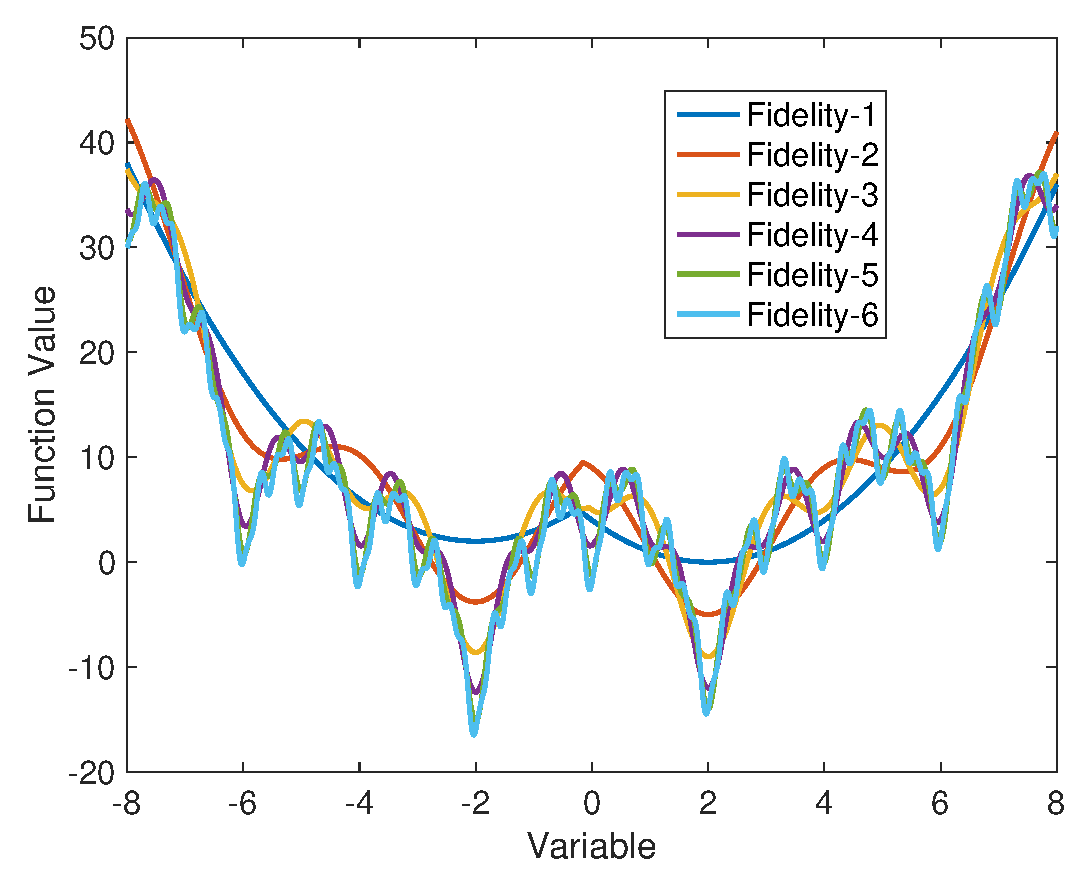
\includegraphics[width=0.2\textwidth,height = 0.14\textheight]{Figures/Figure1.eps}}\quad
	\subfigure[]{\label{fig:emustat}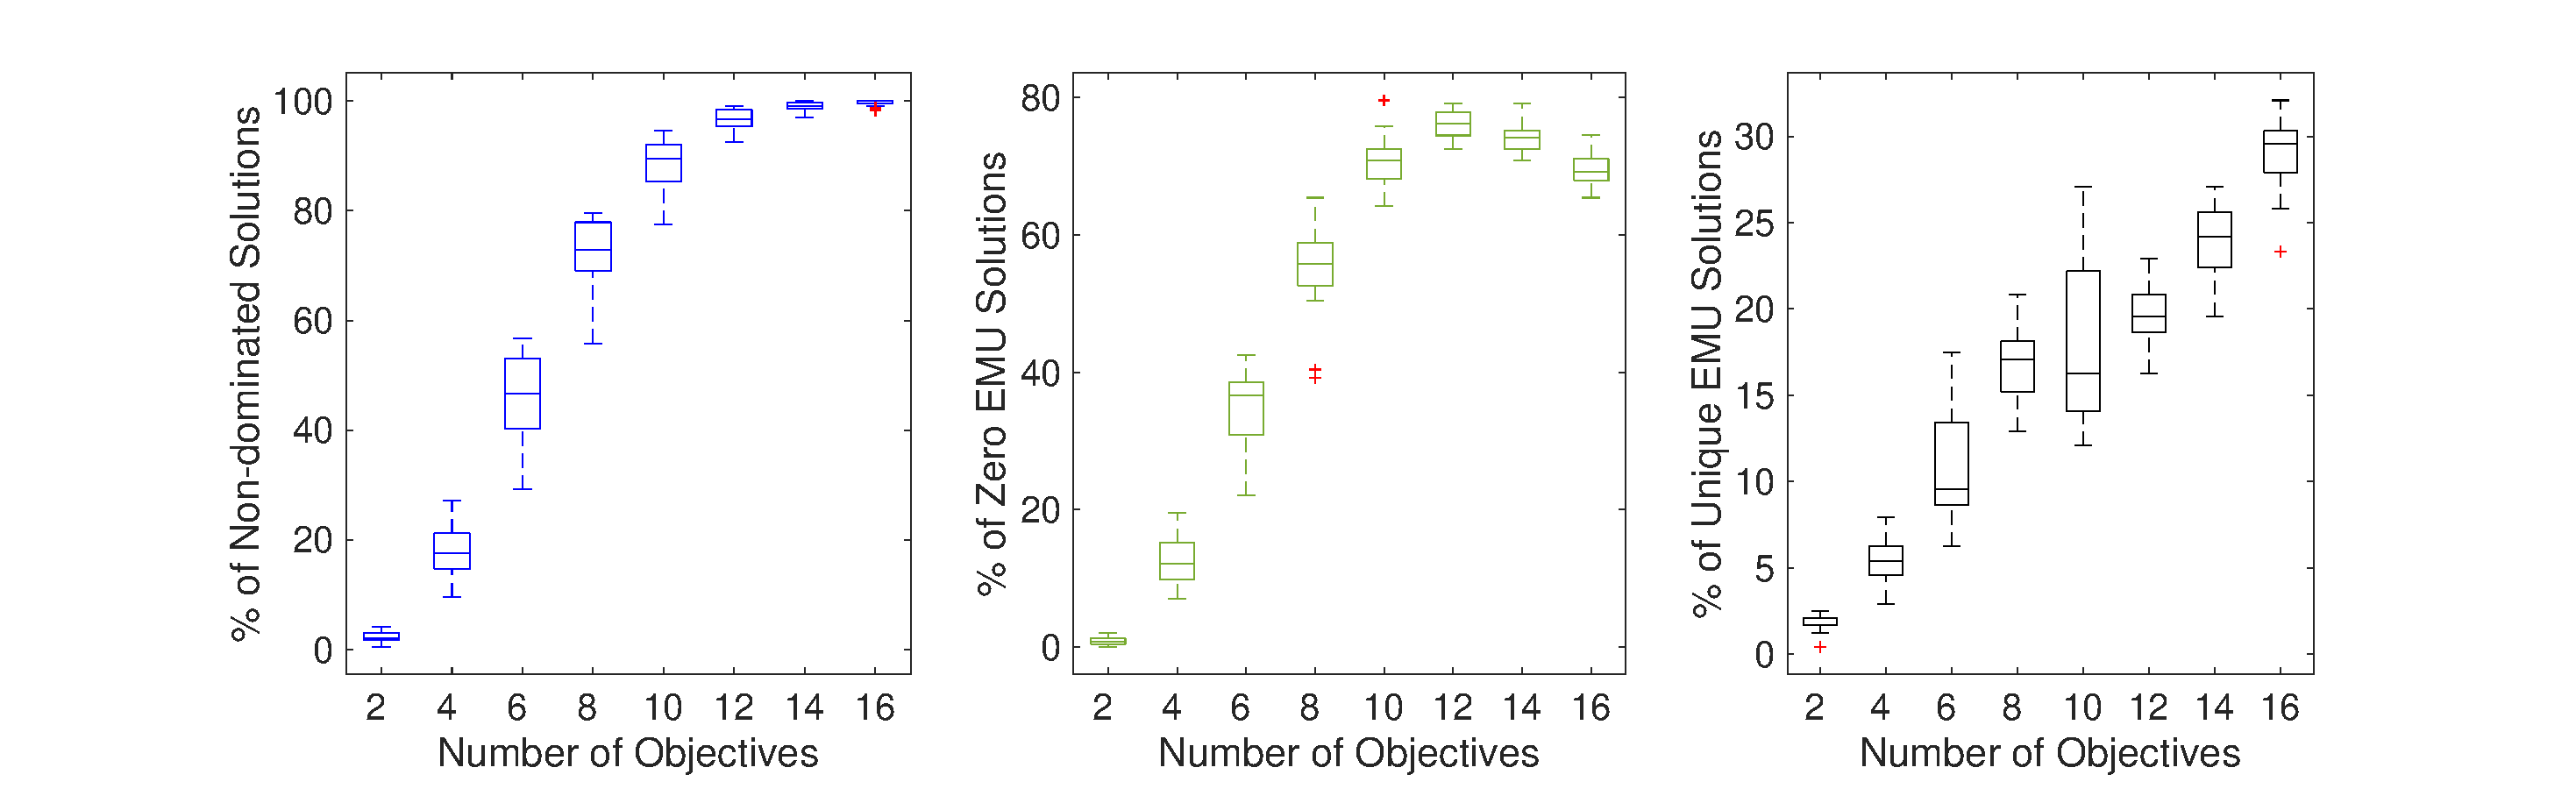
\includegraphics[width=0.7\textwidth,height = 0.15\textheight]{Figures/Figure2.eps}}\quad     
	\caption{(a) Bi-objective test example, (b) Percentage of non-dominated, zero EMU, and unique non-zero EMU solutions}
	\label{fig:testprop}
\end{figure*}

To overcome this limitation, we introduce a new measure, which is based on recursive computation of expected marginal utility. This measure has the benefits of expected marginal utility, while avoiding the problem posed due to identical or zero EMU values. The goal of this process is to obtain $K$ unique, sparse solutions of interest.

\section{Proposed approach}
\label{sec:propmetric}

The proposed approach operates by recursive computation of EMU and is referred to as EMU\textsuperscript{r}. The approach identifies $K$ unique, sparse solutions of interest and is outlined in Algo.~\ref{alg:ISOI}. The key steps are discussed in the following sub-sections.

\begin{algorithm}[!ht]\footnotesize
	\caption{ISOI}
	\show\LOOP
	\textbf{Input:} $NDF$\hspace{1mm}(objective values of all unique nondominated solutions~($P$) for an $m$ objective problem), $K$\hspace{1mm}(number of SOI required)\\
	\textbf{Output:} SOI\textsubscript{f}~(Final $K$ solutions selected)
	\begin{algorithmic}[1]
		\STATE \textbf{Generate} $|W|$~($|W|~\ge~K$) reference directions~($W$).
		\STATE SOI = $\emptyset$, SOI\textsubscript{A} = $P$.
		\WHILE{$|$SOI$|~<~K$} 
		\LCOMMENT{Start \textit{Outer Loop}}
		\WHILE{$|$SOI\textsubscript{A}$|~>~0$} 
		\LCOMMENT{Start \textit{Inner Loop}}
		\STATE \textbf{Compute} EMU\textsuperscript{r} of each solution in SOI\textsubscript{A} using $W$.
		\STATE \textbf{Associate} solutions to their closest reference directions. 
		\STATE \textbf{Identify} solutions with highest EMU\textsuperscript{r} values along each non-empty reference directions. 
		\STATE \textbf{Select} a set of solutions ($S$, $S~\subseteq~$SOI\textsubscript{A}) with higher EMU\textsuperscript{r} values than the neighboring solutions (based on neighboring reference directions).
		\IF{($|S|~\le~K)~\vee~(|S|~=~|$SOI\textsubscript{A}$|)$}
		\BREAK.
		\ELSE
		\STATE SOI\textsubscript{A} = $S$.
		\ENDIF
		\LCOMMENT{End \textit{Inner Loop}}
		\ENDWHILE
		\STATE SOI = SOI~$\cup$~SOI\textsubscript{A}.
		\STATE SOI\textsubscript{A} = $P~\setminus$~SOI.
		\LCOMMENT{End \textit{Outer Loop}}
		\ENDWHILE
		\STATE Order solutions in SOI based on EMU\textsuperscript{r} values.
		\IF{$|$SOI$|~>~K$}
		\STATE Classify solutions of the SOI into three sets: $Internal$, $Peripheral$ and $Peripheral_E$.
		\IF{$|Internal|~>~K$}
		\STATE Pick $K$ diverse $Internal$ solutions to construct SOI\textsubscript{f}.
		\ELSIF{$|Internal|~<~K$}
		\STATE Combine $Internal$ with $K - |Internal|$ diverse solutions from $Peripheral~\cup~Peripheral_E$ to construct SOI\textsubscript{f}.
		\ENDIF
		\ELSIF {$|$SOI$|~=~K$}
		\STATE SOI\textsubscript{f} = SOI.
		\ENDIF
	\end{algorithmic}
	\label{alg:ISOI}
\end{algorithm} 

\subsection{Generate} A structured set $W$ of reference points~($|W|~\ge~K$) is generated spanning a hyperplane with unit intercepts in each objective axis using normal boundary intersection method (NBI) \cite{das1998normal}. The approach generates $|W|$ reference directions by joining reference points to the origin.

\subsection{Compute} In the first stage, the objective values ($NDF$) of all the unique non-dominated solutions~($P$) are scaled using ideal and nadir vectors. The EMU values of all solutions are computed using all reference directions~\cite{branke2004finding} generated in the previous step. The solutions with non-zero EMU values are ordered based on descending values of EMU and assigned to the first ``front''\footnote{Note that this ``front'' is not to be confused with a non-dominated front. All solutions that are given as input to the proposed approach are non-dominated.}. In the next stage, only the solutions having zero EMU values are considered and their EMU values are recomputed using the complete set of reference directions. The solutions with non-zero EMU values in this stage are ordered and assigned to the second front. This process continues until at most one solution has a zero EMU value. Thus, all the solutions can be ordered in each front. Thereafter, maximum EMU value of each front~(starting from the last) is added to the EMU value of all members belonging to the next front. Thus all solutions in the trade-off set would have a non-zero EMU\textsuperscript{r} value.

\subsection{Associate} In the next stage, two measures $d_1$ and $d_2$ are computed for each solution in the scaled objective space. The first measure $d_1$ is the Euclidean distance between origin and the foot of the normal drawn from the solution to a reference direction, while the second measure $d_2$ is the length of the normal~\cite{asafuddoula2014decomposition}. For each solution, the associated reference direction is identified as the one corresponding to its minimum $d_2$ value. 

\subsection{Identify} The above association might result in some directions having no solutions and some others having several solutions associated with them. For each non-empty reference direction, the associated solution with the maximum EMU\textsuperscript{r} value is selected. 

\subsection{Select} At the end of identification stage, there could still be potentially a large number of solutions selected~(e.g. if one solution has been selected along each reference direction). To narrow down the selection further, for any given solution along a non-empty reference direction, all solutions associated with its immediate neighboring reference directions are compared based on EMU\textsuperscript{r} measure. If the solution along the original non-empty reference direction is still the best following the neighborhood comparison, this solution is selected. Otherwise, no solution is selected as the best for this comparison. Please take note that EMU\textsuperscript{r} values are not recomputed during the comparison and the order of comparison does not affect the selection since none of the solutions are deleted. The process is repeated for every non-empty reference direction to construct the most preferred set of solutions (SOI\textsubscript{A}). 


If the number of solutions in SOI\textsubscript{A} is more than $K$, the above processes (\textit{Inner Loop}) continue until cardinality of the set SOI\textsubscript{A} does not change or is less than $K$. At the end of the \textit{Inner Loop}, the members in SOI\textsubscript{A} are used to construct SOI. 

The \textit{Outer Loop} starts if SOI contains fewer than $K$ solutions. In this loop, SOI\textsubscript{A} is set to contain the remaining solutions in $P$, i.e, $P~\setminus~$SOI and the \textit{Inner Loop} continues until the cardinality of the set SOI reaches at least $K$.

At the end of both the loops, the reduction stage begins if SOI contains more than $K$ solutions. In this stage, solutions belonging to SOI are further divided into three classes: $Peripheral_E$, $Peripheral$  and $Internal$. Solutions having at least one objective at its minimum value among the non-dominated solutions belong to the $Peripheral_E$ class. Solutions closest to the reference directions passing through the edges of the hyperplane belong to the $Peripheral$ class. The remaining solutions belong to the $Internal$ class. Based on the number of solutions in SOI at this step, two cases can occur:  

\begin{itemize}
	\item If the set $|$SOI$|~>~K$, the number of solutions belonging to the class $Internal$ is observed. If the number exceeds $K$, then $K$ diverse solutions are picked from $Internal$ class using affinity propagation clustering \cite{apcluster2011}. In the event the $Internal$ class contains fewer than $K$ solutions, $K - |Internal|$ solutions are picked from other classes using affinity propagation clustering \cite{apcluster2011}. Solutions belonging to the $Internal$ class are preferred over the solutions belonging to $Peripheral$ and $Peripheral_E$ class since prior studies have indicated that the decision makers tend to prefer solutions from the middle section of the POF, to avoid extreme objective values~\cite{das_characterizing_1999}. The picked solutions are combined to form the final SOI\textsubscript{f}.
	
	\item If SOI contains exactly $K$ points, then SOI\textsubscript{f} = SOI.
\end{itemize}

For the bi-objective test example consisting of 150 unique non-dominated solutions in Fig.~\ref{fig:soitest}, 75 reference directions were used to compute EMU\textsuperscript{r} and EMU of all solutions. Fig.~\ref{fig:test} shows the effectiveness of the proposed approach compared to other measures~(EMU, convex bulge and HV contribution) in choosing a required number~($K=9$) of solutions. One can see that EMU, convex bulge and hypervolume measures could not identify all the SOIs ($A$, $B$, $C$, $E$, $G$, $I$ and $J$) for the bi-objective test problem. However EMU\textsuperscript{r} measure was able to identify all of them. In this example, SOI contained 15 solutions before the reduction stage. Out of these, 1 solution belonged to $Peripheral_E$, 2 to $Peripheral$ class and 12 to $Internal$ class. Therefore the final SOI set SOI\textsubscript{f} contains 9 solutions from the $Internal$ class only. For the other indicators~(EMU, Convex bulge and HV contribution), the top 9 solutions were chosen based on descending order of the measure values. It is interesting to note that using the proposed approach all the SOIs were identified before the reduction stage. However, due to the preference for internal SOIs, all the final SOIs belonging to SOI\textsubscript{f} were chosen from the $Internal$ class. 

\begin{figure*}[!htb]
	\centering    
	\subfigure[]{\label{fig:remu}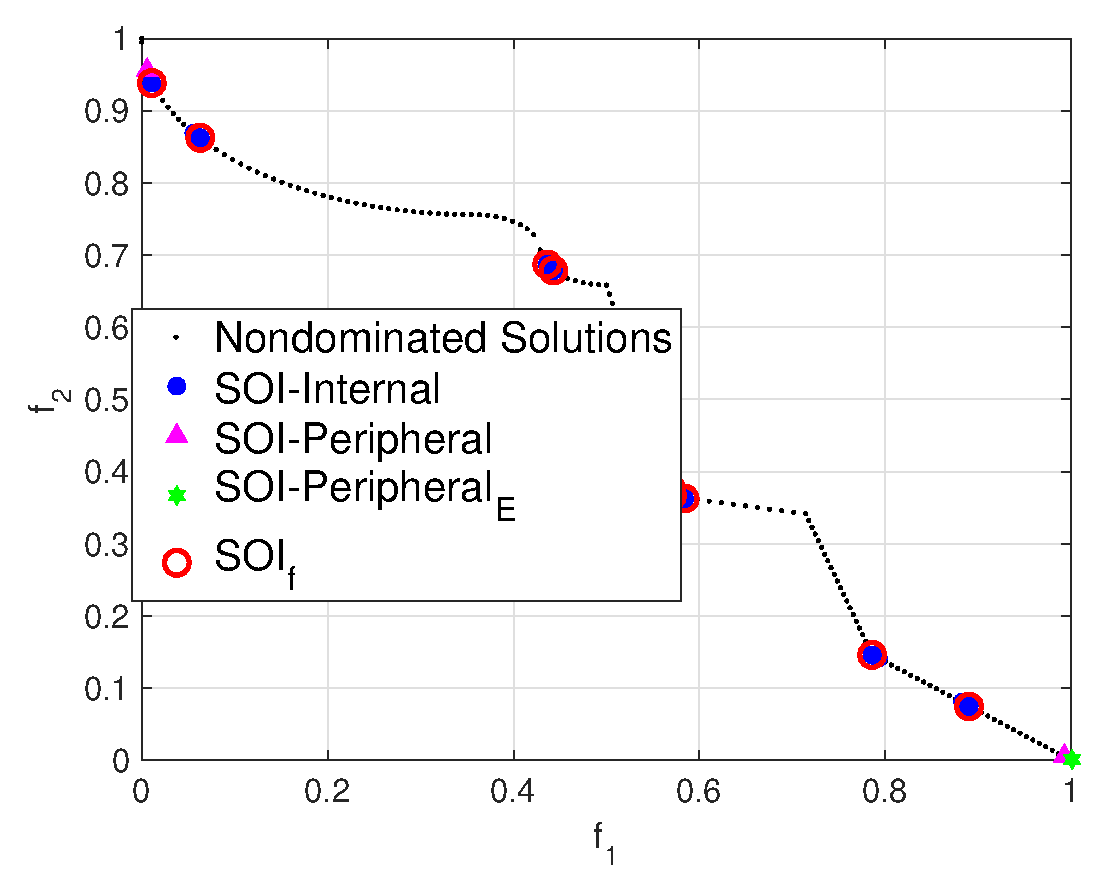
\includegraphics[width=0.21\textwidth]{Figures/Figure3.eps}}\quad
	\subfigure[]{\label{fig:emu}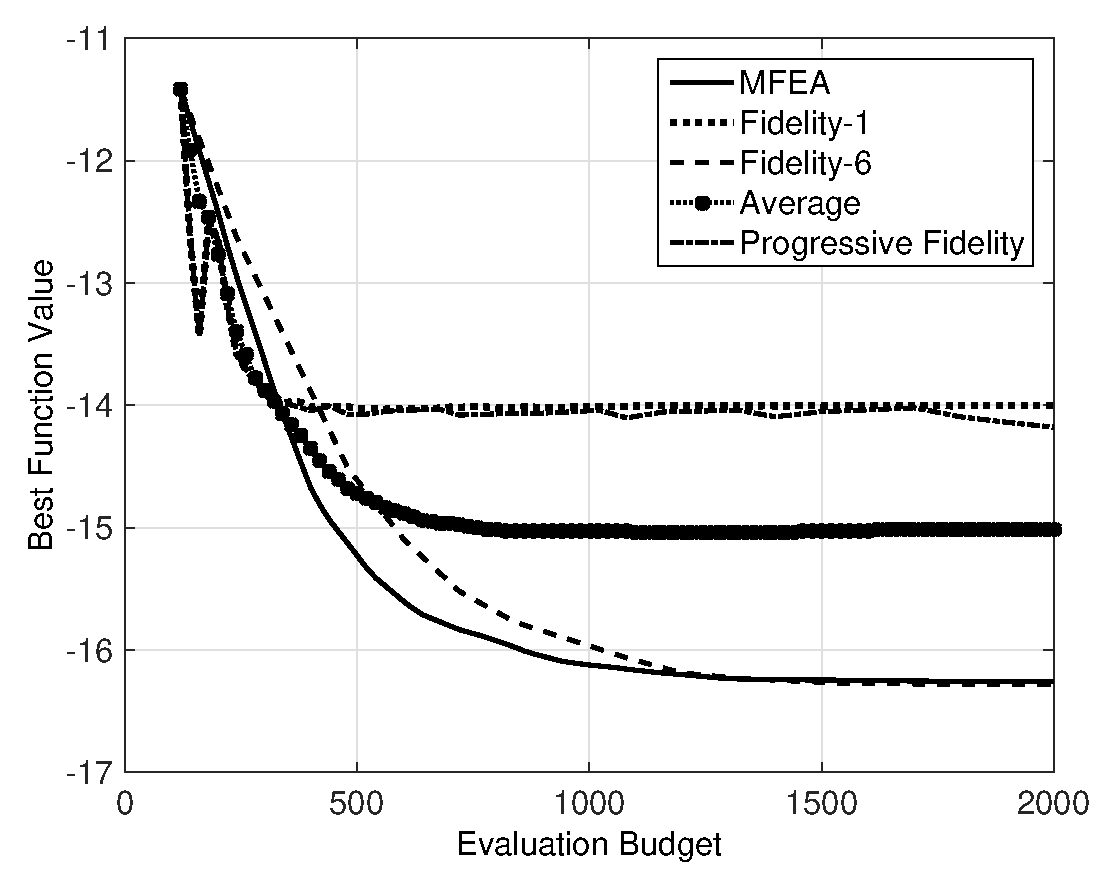
\includegraphics[width=0.21\textwidth]{Figures/Figure4.eps}}\quad
	\subfigure[]{\label{fig:hyp}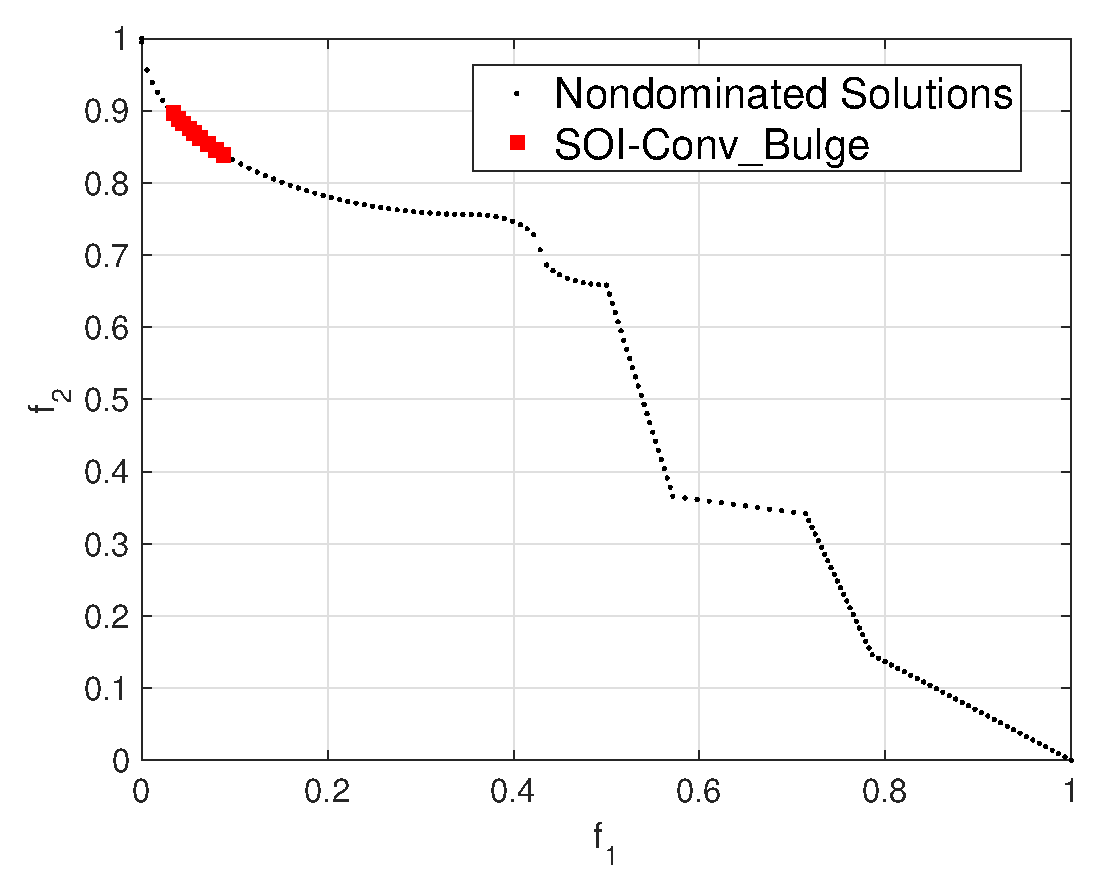
\includegraphics[width=0.21\textwidth]{Figures/Figure5.eps}}\quad
	\subfigure[]{\label{fig:hv}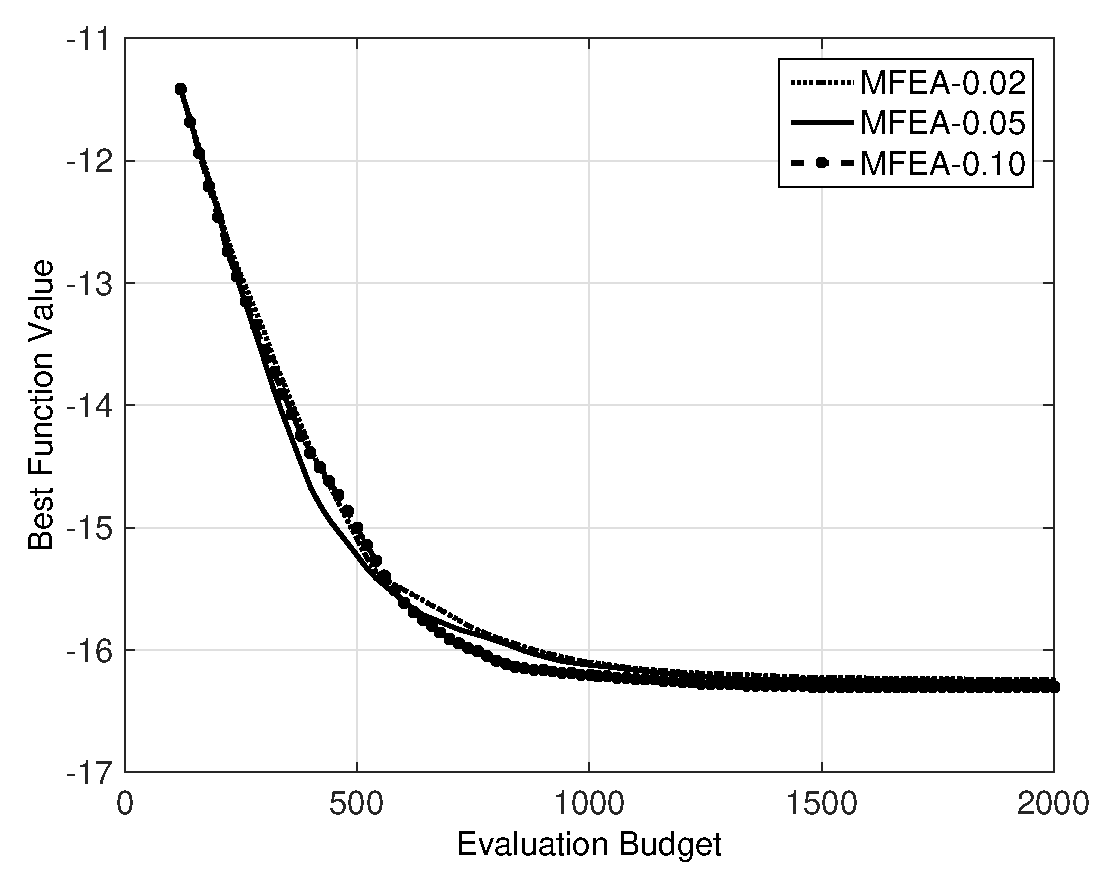
\includegraphics[width=0.21\textwidth]{Figures/Figure6.eps}}\quad      
	\caption{Bi-objective test example: (a) EMU\textsuperscript{r}, (b) EMU, (c) Convex Bulge, (d) HV contribution}
	\label{fig:test}
\end{figure*}


\section{Numerical experiments}
\label{sec:numex} 

We assess the performance of the proposed approach using two more bi-objective benchmarks~(DO2DK and DEB2DK \cite{branke2004finding}), one 3-objective benchmark~(DEB3DK \cite{branke2004finding}) and two practical engineering problems~(Radar Waveform Design~\cite{hughes2007radar} and General Aviation Aircraft~\cite{Simpson1996}) that have been extensively used in many-objective optimization literature. The examples show interesting differences in the SOIs selected based on different approaches. We assume that a decision maker requires $K=9$ solutions following the upper bound of rule of thumb~($7\pm 2$). To enable other researchers to compare with our results, the datasets corresponding to all the problems and the MATLAB code have been made publicly available~\cite{benchmark}.

\subsection{Benchmark problems}

\subsubsection{DO2DK}
In this bi-objective example~\cite{branke2004finding}, the given dataset consists of 200 unique non-dominated solutions. The problem has a skewed POF with 4 knee regions. Fig.~\ref{fig:do2dkplot} shows that both EMU and EMU\textsuperscript{r} were able to discover all knees. However, our approach was able to discover 24 distinct sparse points~(based on the resolution of the 100 reference directions) in SOI set at the end of both the loops. Out of these 24 solutions, one solution belonged to $Peripheral_E$ class~(minimum value in second objective) and all the rest belonged to $Internal$ class. Since internal solutions are preferred, the reduction stage involved picking 9 diverse solutions out of 23 solutions belonging to $Internal$ class. Convex bulge and HV contribution based measures were only able to identify one and three knee regions respectively.

\begin{figure*}[!htb]
	\centering    
	\subfigure[]{\label{fig:remudo2}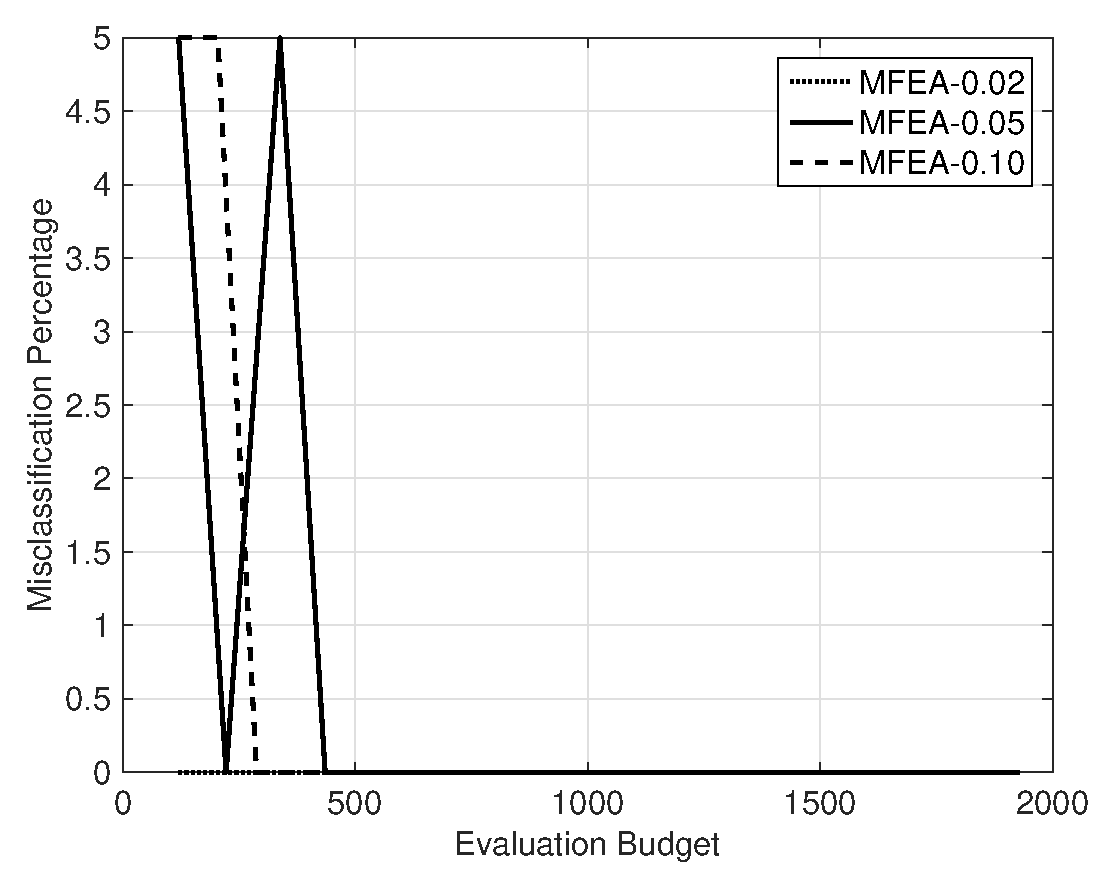
\includegraphics[width=0.21\textwidth]{Figures/Figure7.eps}}\quad
	\subfigure[]{\label{fig:emudo2}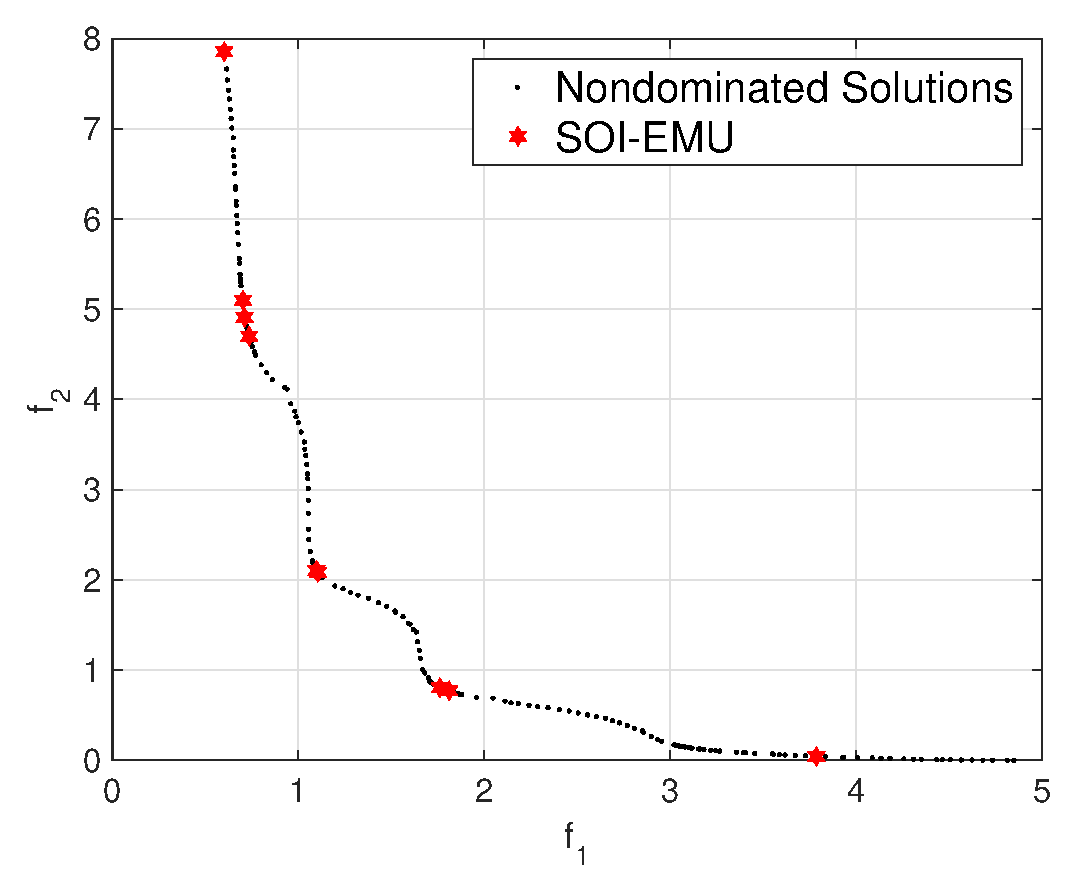
\includegraphics[width=0.21\textwidth]{Figures/Figure8.eps}}\quad
	\subfigure[]{\label{fig:hypdo2}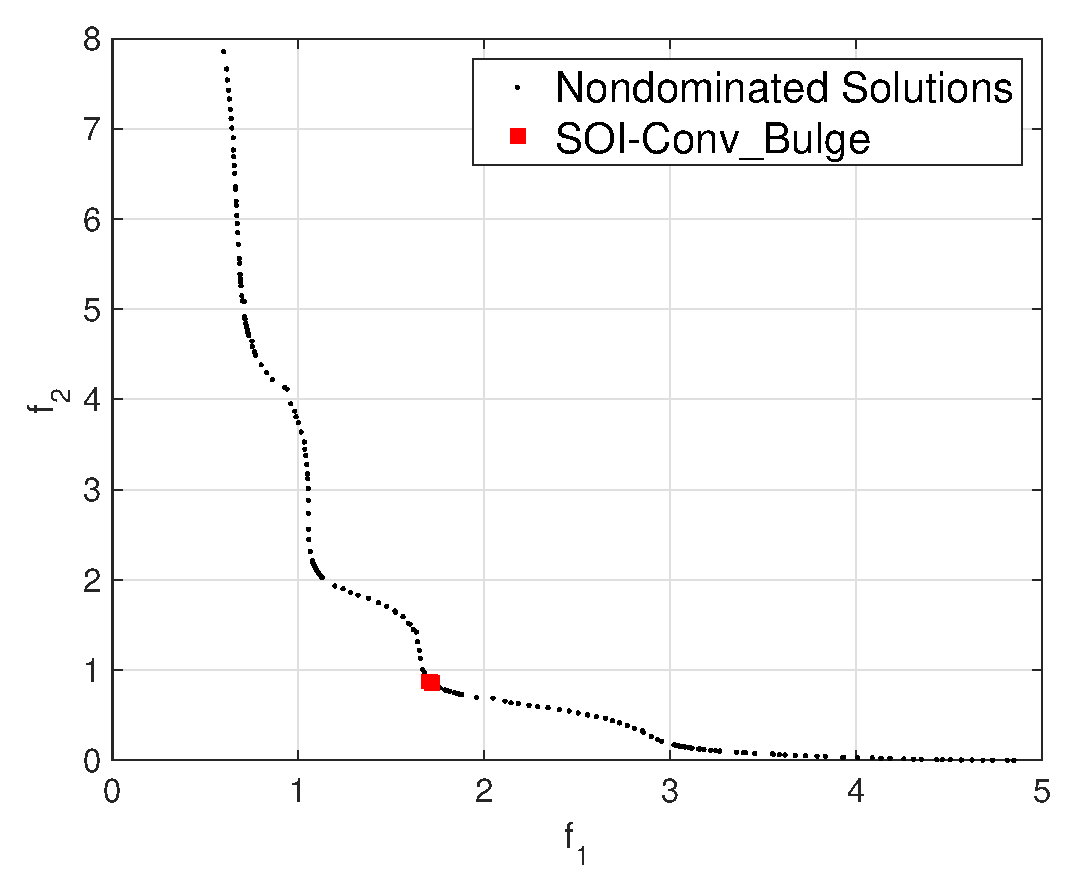
\includegraphics[width=0.21\textwidth]{Figures/Figure9.eps}}\quad
	\subfigure[]{\label{fig:hvdo2}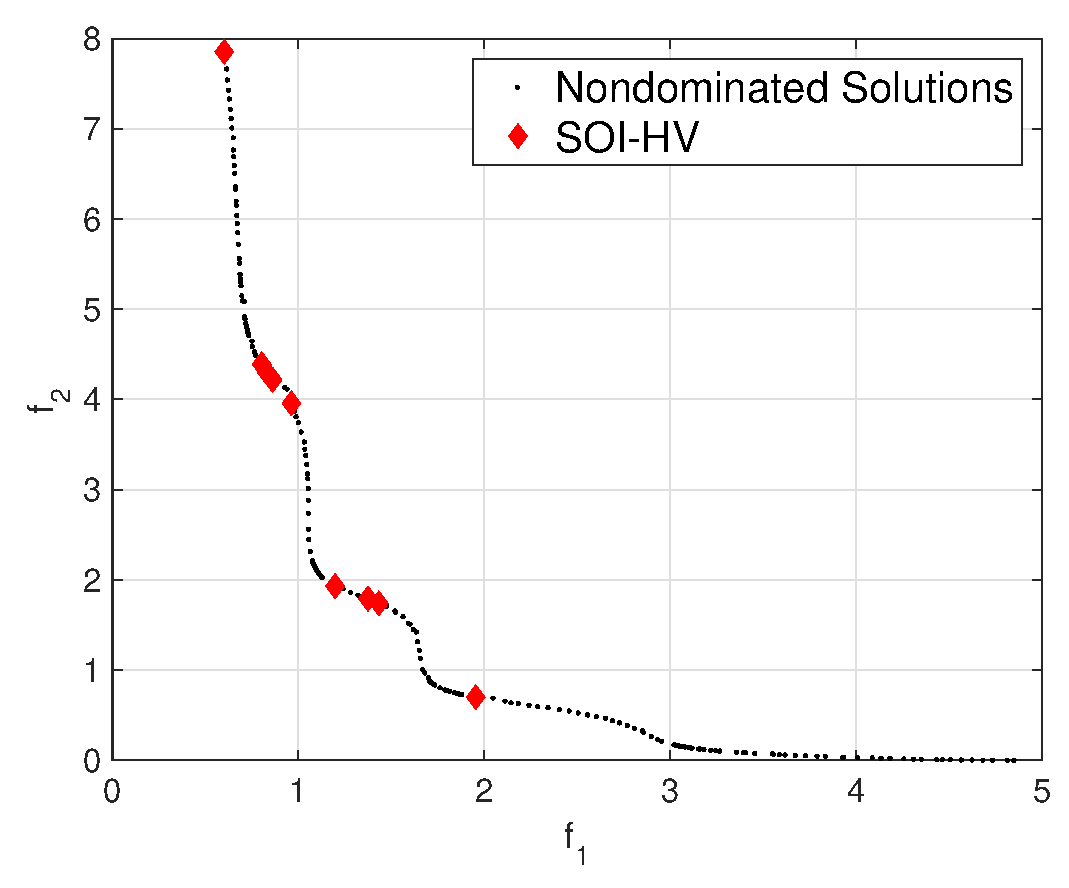
\includegraphics[width=0.21\textwidth]{Figures/Figure10.eps}}\quad      
	\caption{DO2DK with 4 knee regions: (a) EMU\textsuperscript{r}, (b) EMU, (c) Convex Bulge, (d) HV contribution}
	\label{fig:do2dkplot}
\end{figure*}

\subsubsection{DEB2DK}
The DEB2DK problem \cite{branke2004finding} is similar to DO2DK, but it is concave near the extremities of the POF, and has 4 knee regions. The given dataset consists of 200 unique non-dominated solutions. Both EMU and EMU\textsuperscript{r} were able to locate all of them, whereas convex bulge and HV contribution could only identify two of them. Fig.~\ref{fig:deb2dkplot} shows the difference in SOIs obtained using the different methods. 100 reference directions were used to compute EMU\textsuperscript{r} and EMU. Out of the 14 solutions belonging to SOI (before the reduction stage), 2 belonged to the $Peripheral_E$ class, 2 to $Peripheral$ class and the rest to $Internal$ class. Fig.~\ref{fig:remudeb2} shows the final SOIs, which were picked from the $Internal$ class. 

\begin{figure*}[!htb]
	\centering    
	\subfigure[]{\label{fig:remudeb2}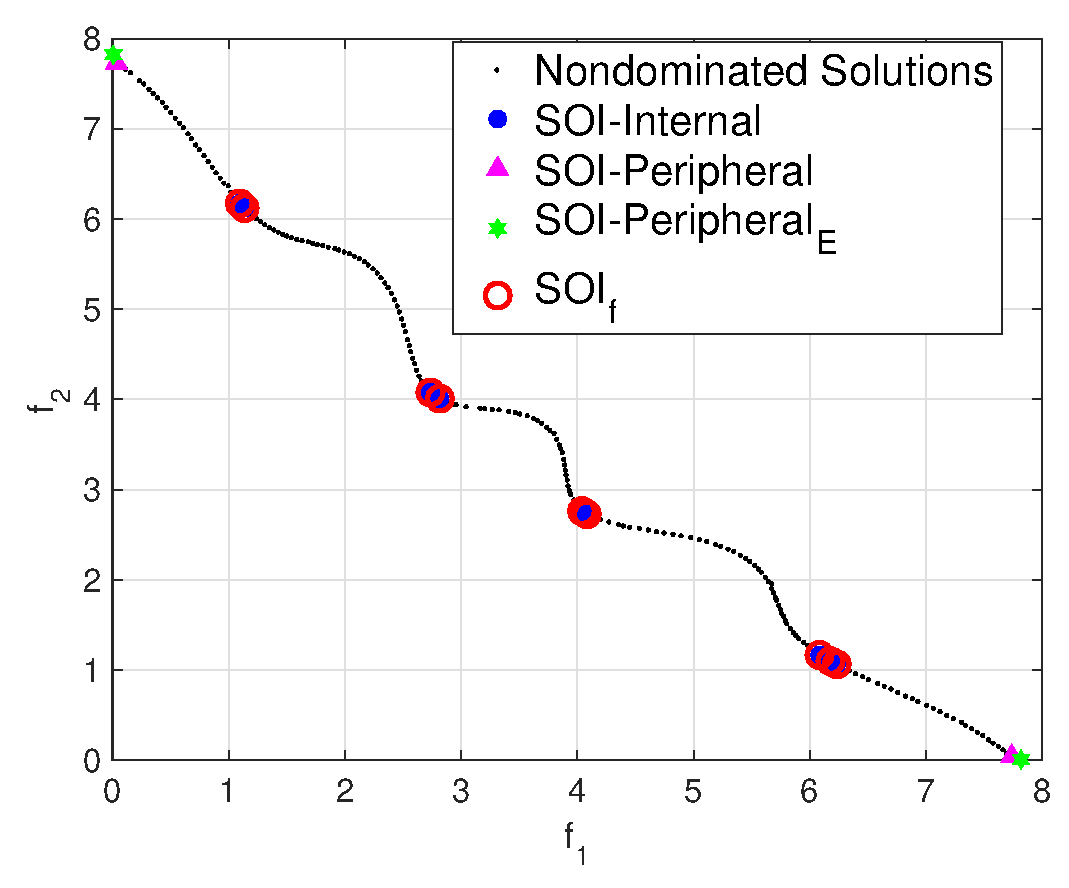
\includegraphics[width=0.21\textwidth]{Figures/Figure11.eps}}\quad
	\subfigure[]{\label{fig:emudeb2}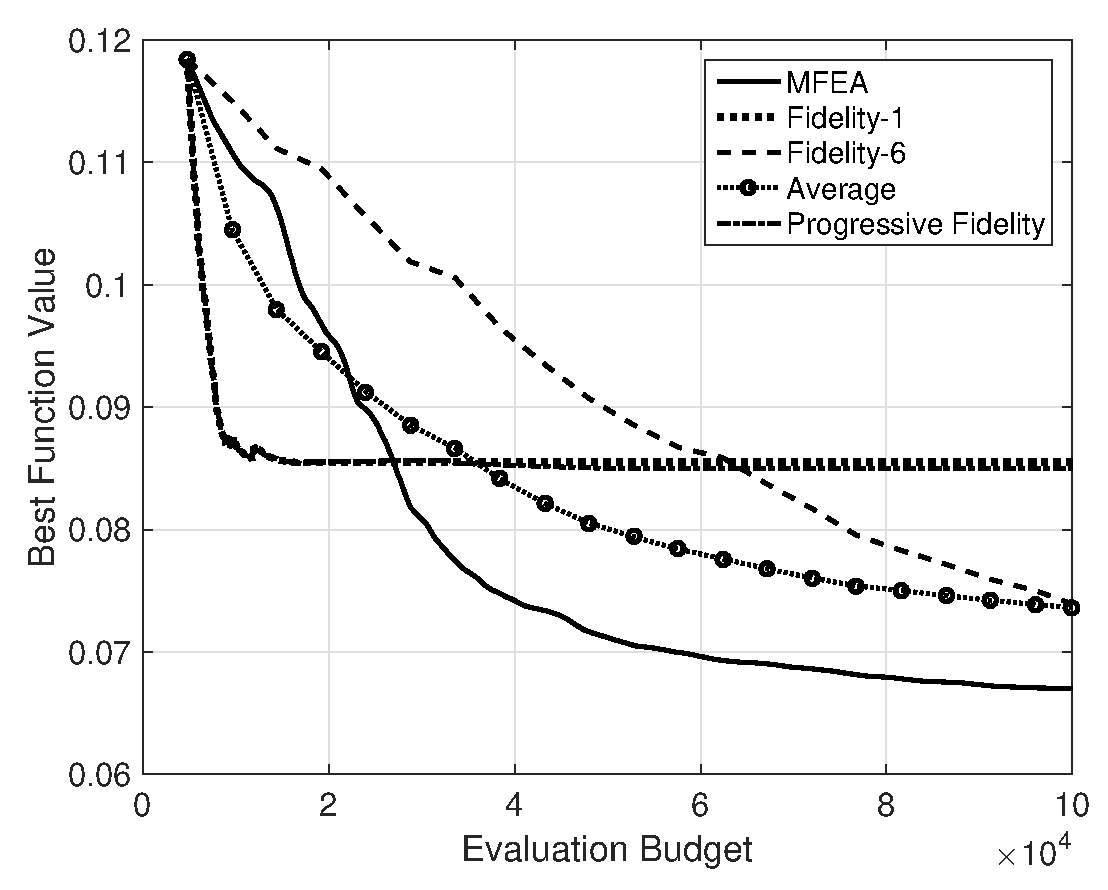
\includegraphics[width=0.21\textwidth]{Figures/Figure12.eps}}\quad
	\subfigure[]{\label{fig:hypdeb2}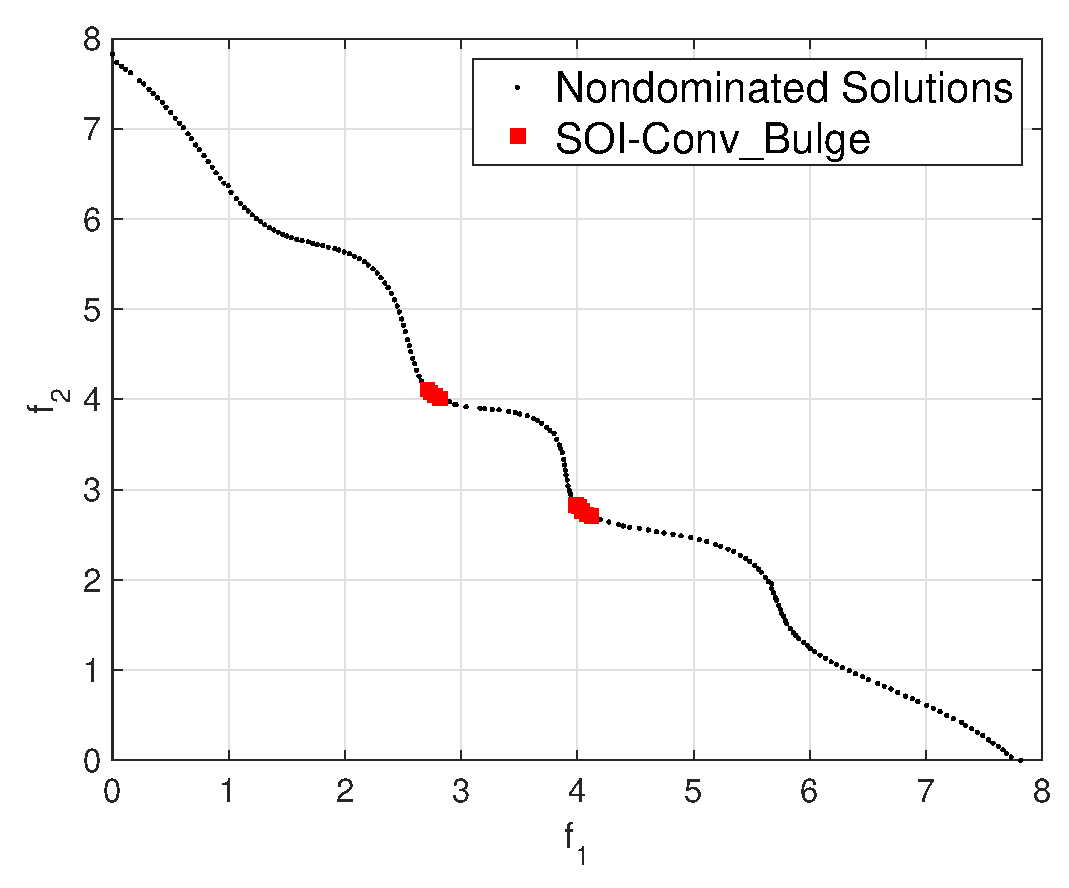
\includegraphics[width=0.21\textwidth]{Figures/Figure13.eps}}\quad
	\subfigure[]{\label{fig:hvdeb2}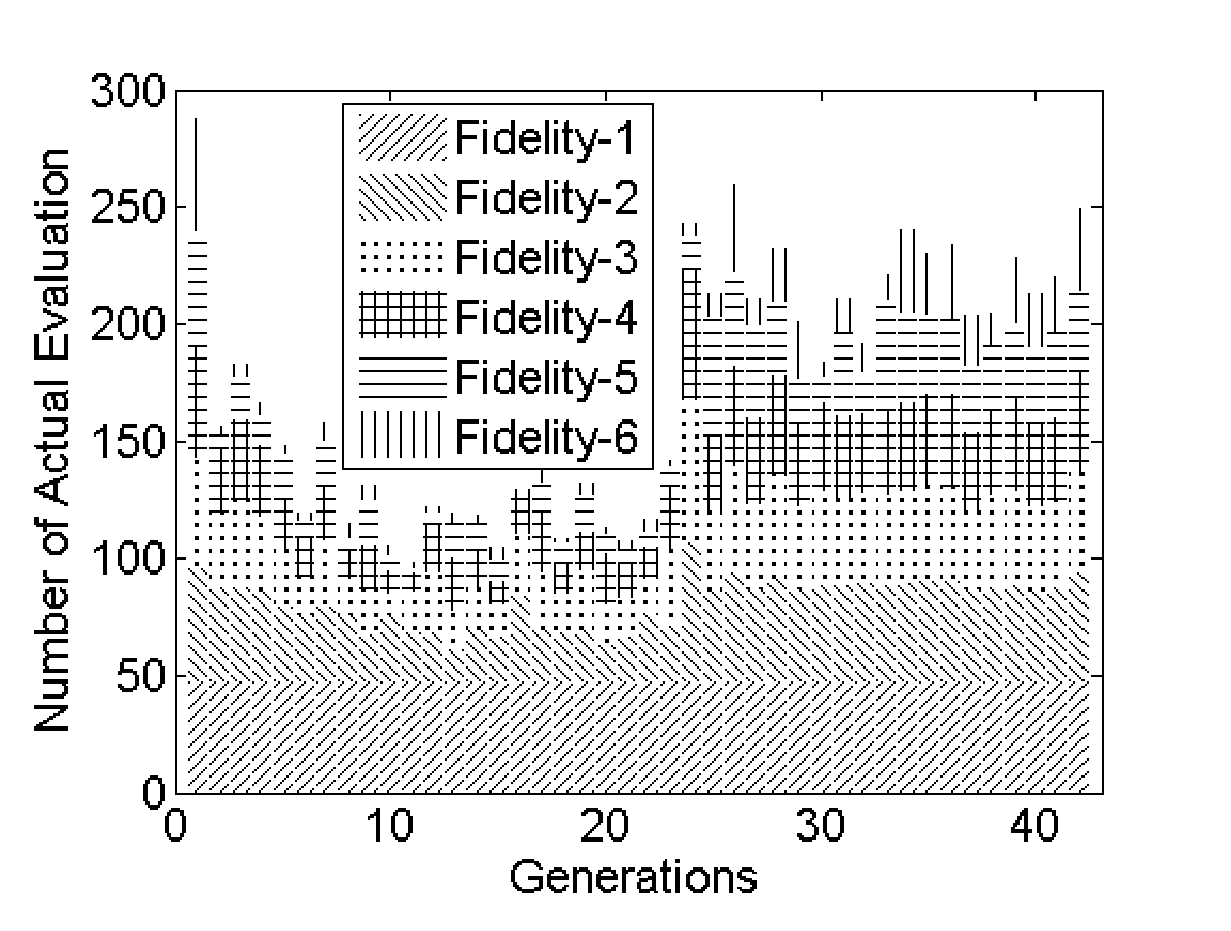
\includegraphics[width=0.21\textwidth]{Figures/Figure14.eps}}\quad     
	\caption{DEB2DK with 4 knee regions: (a) EMU\textsuperscript{r}, (b) EMU, (c) Convex Bulge, (d) HV contribution}
	\label{fig:deb2dkplot}
\end{figure*}

\subsubsection{DEB3DK}

For this 3-objective problem~\cite{branke2004finding}, two versions, with one and four knees, were studied. 300 reference directions were used for EMU\textsuperscript{r} and EMU computations for both the instances. Fig.~\ref{fig:deb3dk1plot} and Fig.~\ref{fig:deb3dk4plot} show the performance on the instances with one and four knee regions, respectively. 

\begin{figure*}[!htb]
	\centering    
	\subfigure[]{\label{fig:remudeb31}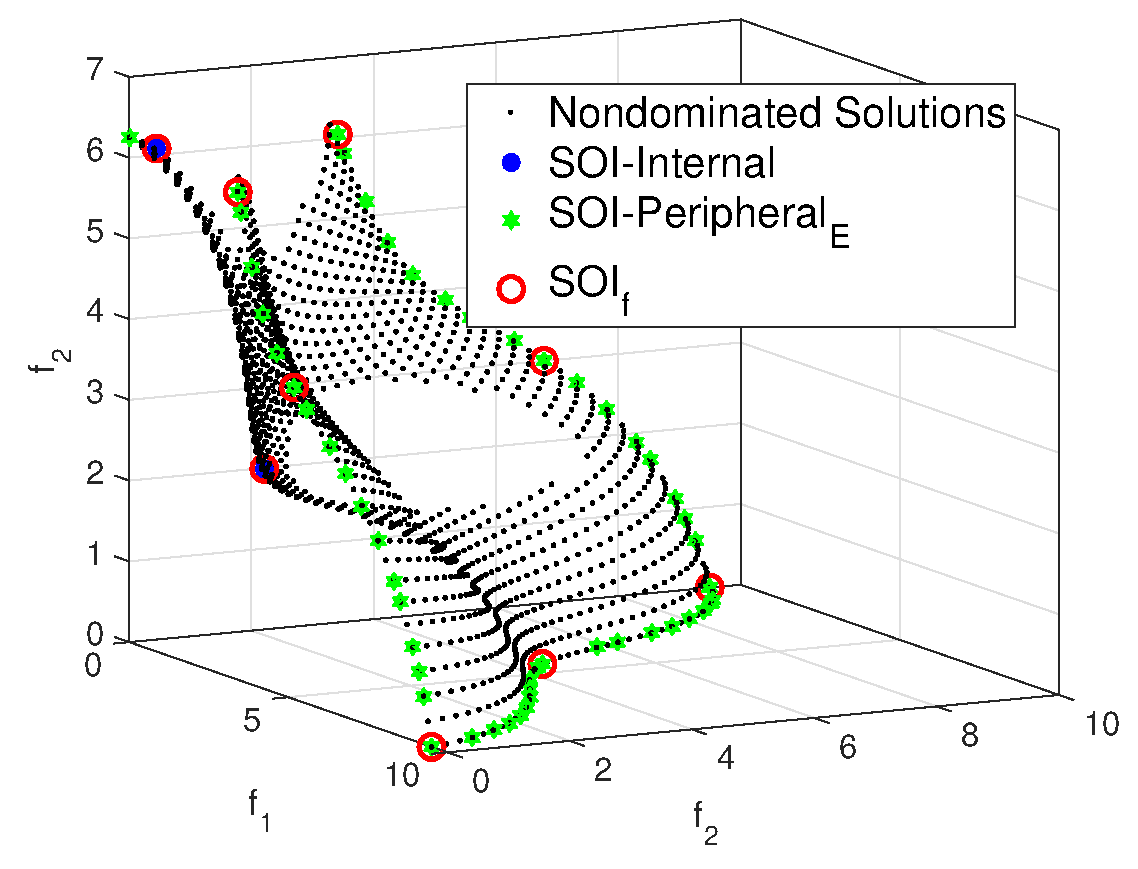
\includegraphics[width=0.21\textwidth]{Figures/Figure15.eps}}\quad
	\subfigure[]{\label{fig:emudeb31}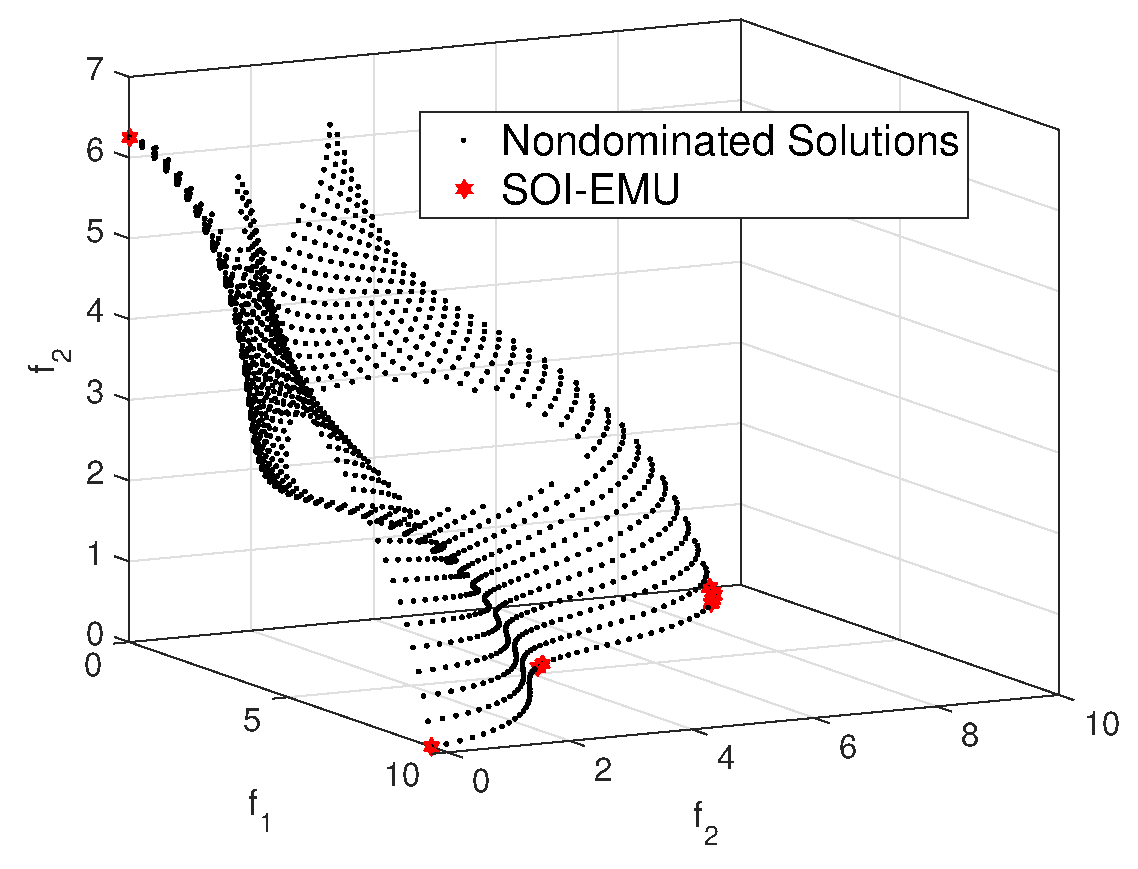
\includegraphics[width=0.21\textwidth]{Figures/Figure16.eps}}\quad
	\subfigure[]{\label{fig:hypdeb31}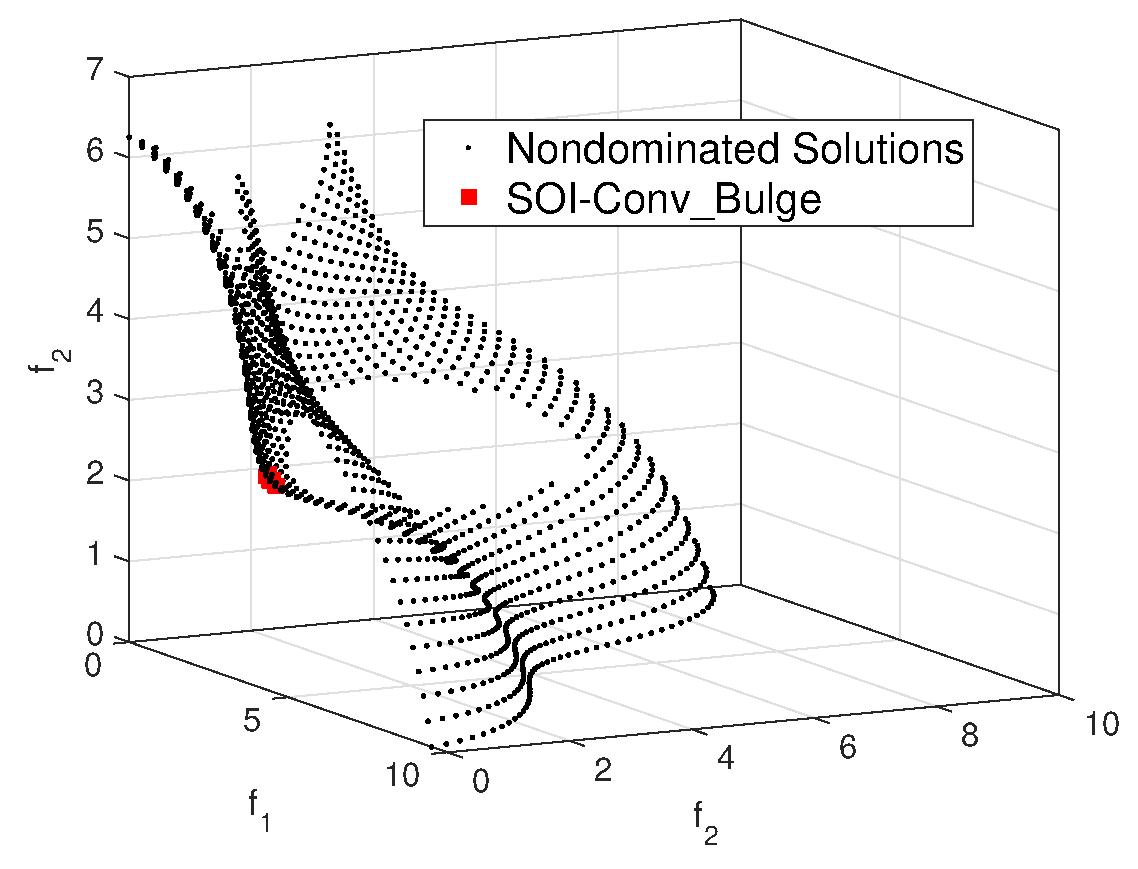
\includegraphics[width=0.21\textwidth]{Figures/Figure17.eps}}\quad
	\subfigure[]{\label{fig:hvdeb31}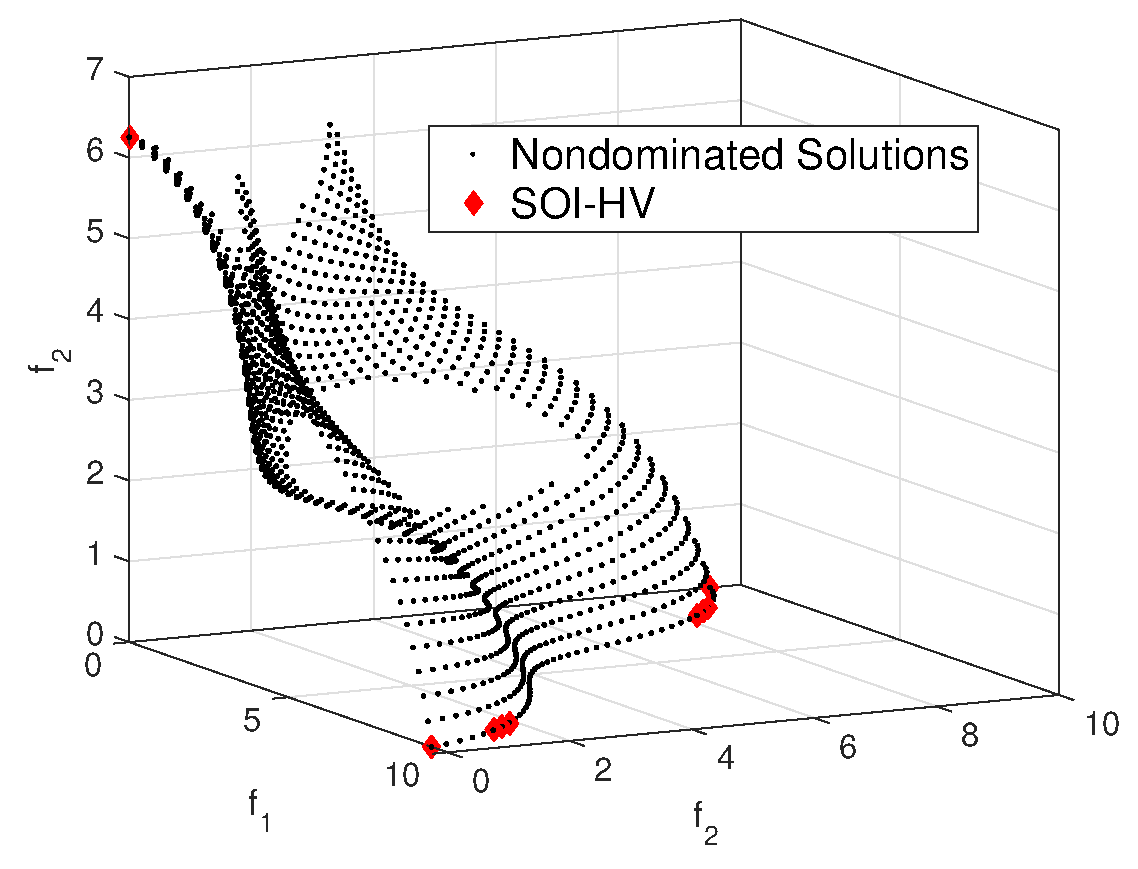
\includegraphics[width=0.21\textwidth]{Figures/Figure18.eps}}\quad 
	\caption{DEB3DK with 1 knee region: (a) EMU\textsuperscript{r}, (b) EMU, (c) Convex Bulge, (d) HV contribution}
	\label{fig:deb3dk1plot}
\end{figure*}

For DEB3DK with one knee region~(1520 unique non-dominated solutions initially), both EMU and HV contribution based measures failed to identify the correct knee region, whereas convex bulge based measure was successful. Our approach was able to find 55 solutions in SOI before reduction. Out these, only 2 belonged to $Internal$ class and rest belonged to $Peripheral_E$ class. In the final set of 9 solutions belonging to the SOI\textsubscript{f} set, 2 solutions belonging to the $Internal$ class were preserved and 7 diverse solutions were picked from 53 solutions belonging to the $Peripheral_E$ class of SOI. 

\begin{figure*}[!htb]
	\centering    
	\subfigure[]{\label{fig:remudeb3}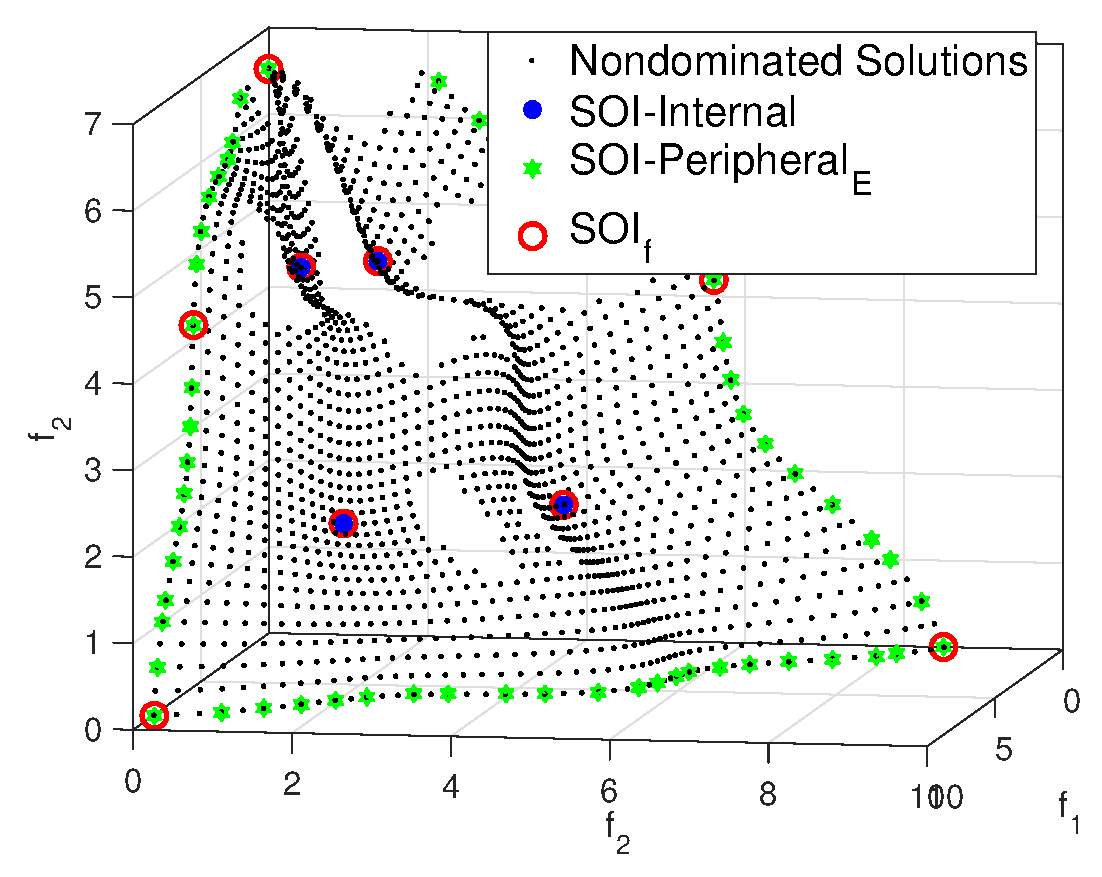
\includegraphics[width=0.21\textwidth]{Figures/Figure19.eps}}\quad
	\subfigure[]{\label{fig:emudeb3}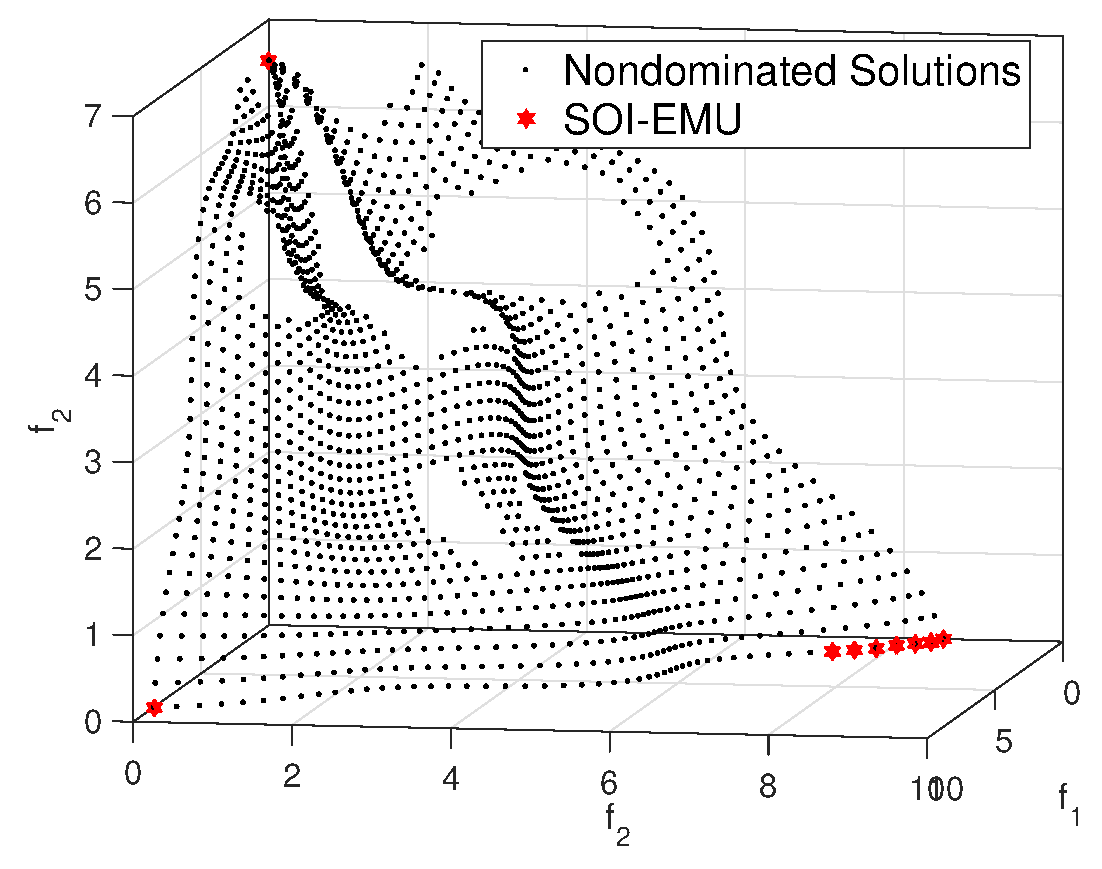
\includegraphics[width=0.21\textwidth]{Figures/Figure20.eps}}
	\subfigure[]{\label{fig:hypdeb3}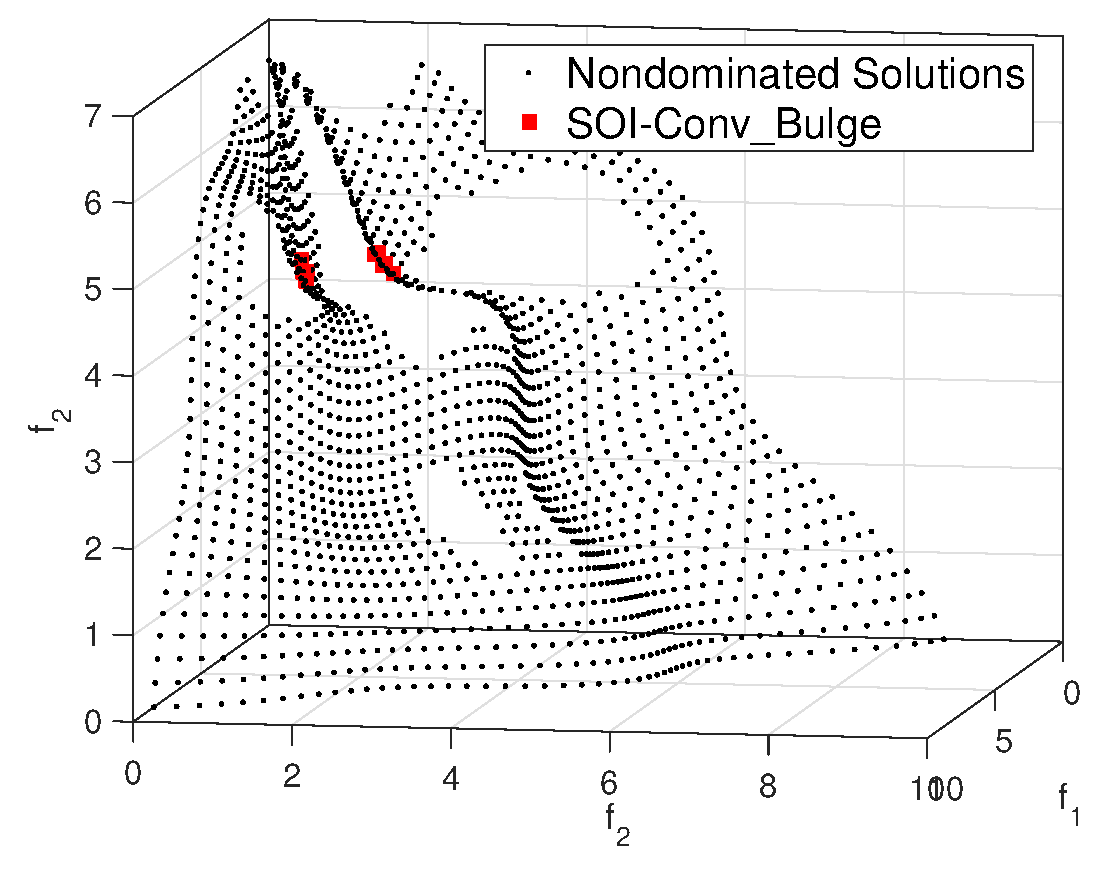
\includegraphics[width=0.21\textwidth]{Figures/Figure21.eps}}\quad
	\subfigure[]{\label{fig:hvdeb3}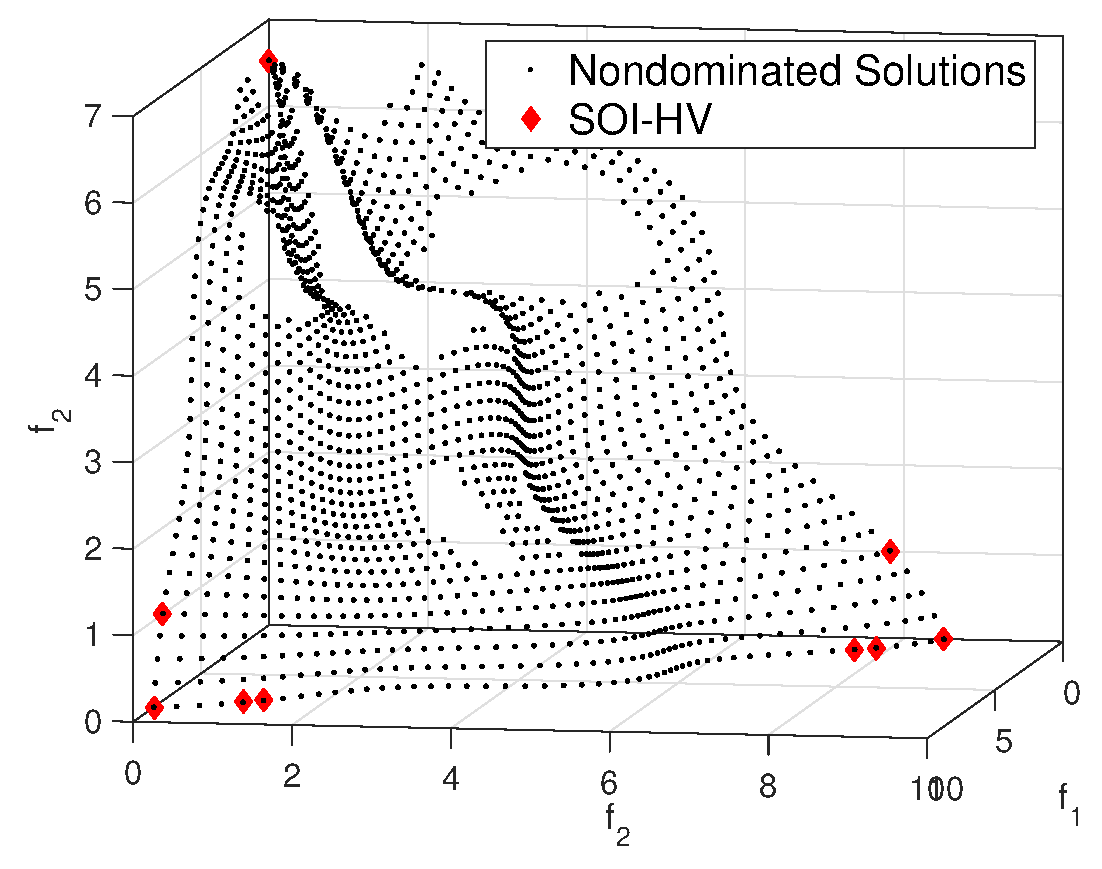
\includegraphics[width=0.21\textwidth]{Figures/Figure22.eps}}\quad       
	\caption{DEB3DK with 4 knee regions: (a) EMU\textsuperscript{r}, (b) EMU, (c) Convex Bulge, (d) HV contribution}
	\label{fig:deb3dk4plot}
\end{figure*}

For DEB3DK instance with 4 knee regions~(1612 unique non-dominated solutions initially), both EMU and HV contribution based measures again failed to identify the 4 knee regions. On the other hand, using convex bulge as a measure, two out of four knee regions were obtained. The proposed approach was able to find all four knee regions in the $Internal$ class in addition to 57 edge solutions~($Peripheral_E$) of the non-dominated front in SOI before reduction. To obtain a total of 9 solutions in SOI\textsubscript{f} set, 5 diverse solutions were selected from the 57 solutions belonging to $Peripheral_E$ class. 

\subsection{Engineering examples}       
\subsubsection{Radar waveform design}
Having demonstrated the performance of the proposed approach for benchmark problems, we now investigate its performance on a nine-objective radar waveform design problem~\cite{hughes2007radar}. The initial set for the problem consists of the solutions obtained from \cite{radarevan}. There are 276,475 data points out of which 100,070 are non-dominated and unique. A total of 3003 reference directions were considered to compute EMU\textsuperscript{r} and EMU for all the solutions. Fig.~\ref{fig:radarplot} represents the SOI obtained using different approaches (except HV contribution based measure since it is computationally prohibitive for such huge number of data points with 9 objectives). The observations are summarized below:

\begin{figure*}[!htb]
	\centering    
	\subfigure[]{\label{fig:remurad}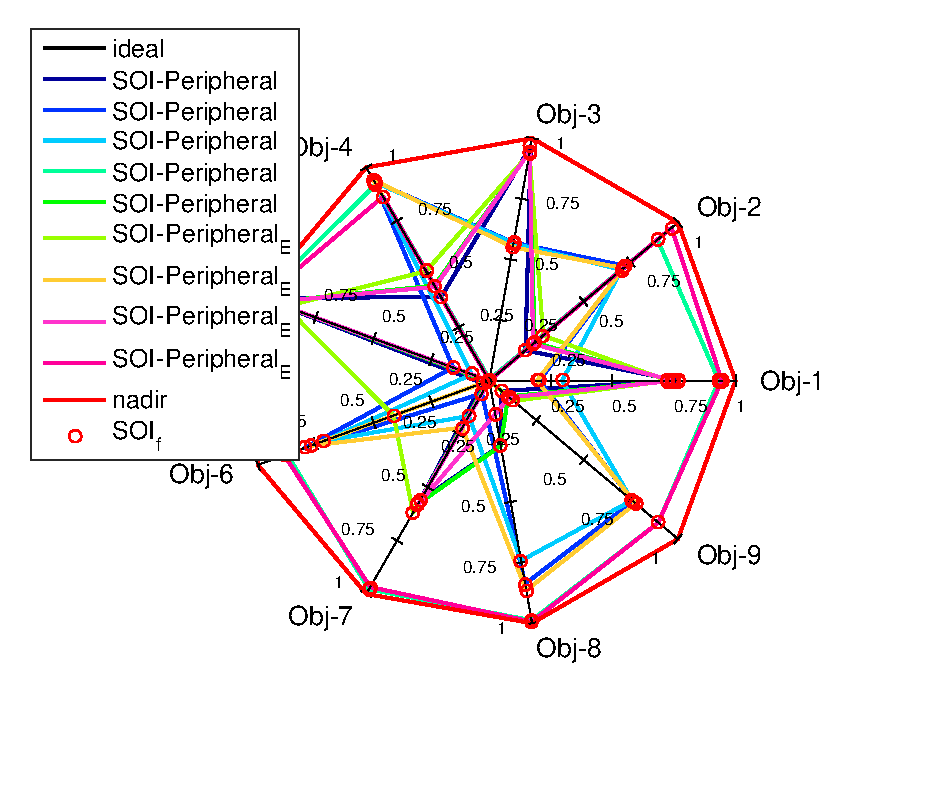
\includegraphics[width=0.37\textwidth]{Figures/Figure23.eps}}
	\subfigure[]{\label{fig:emurad}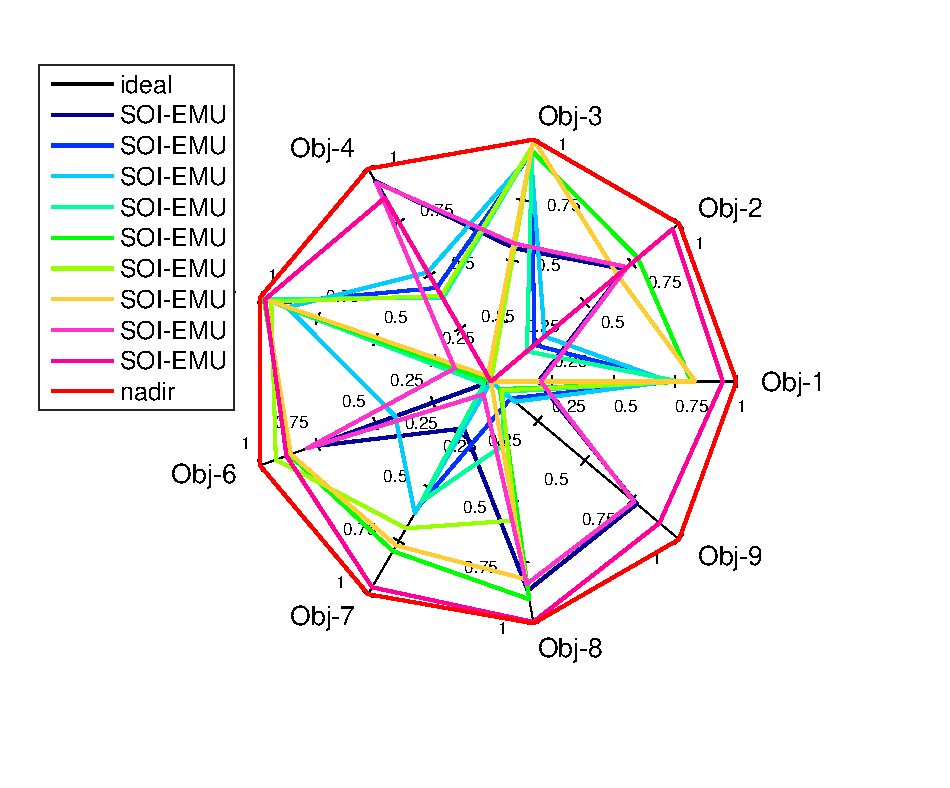
\includegraphics[width=0.37\textwidth]{Figures/Figure24.eps}}
	\subfigure[]{\label{fig:hyprad}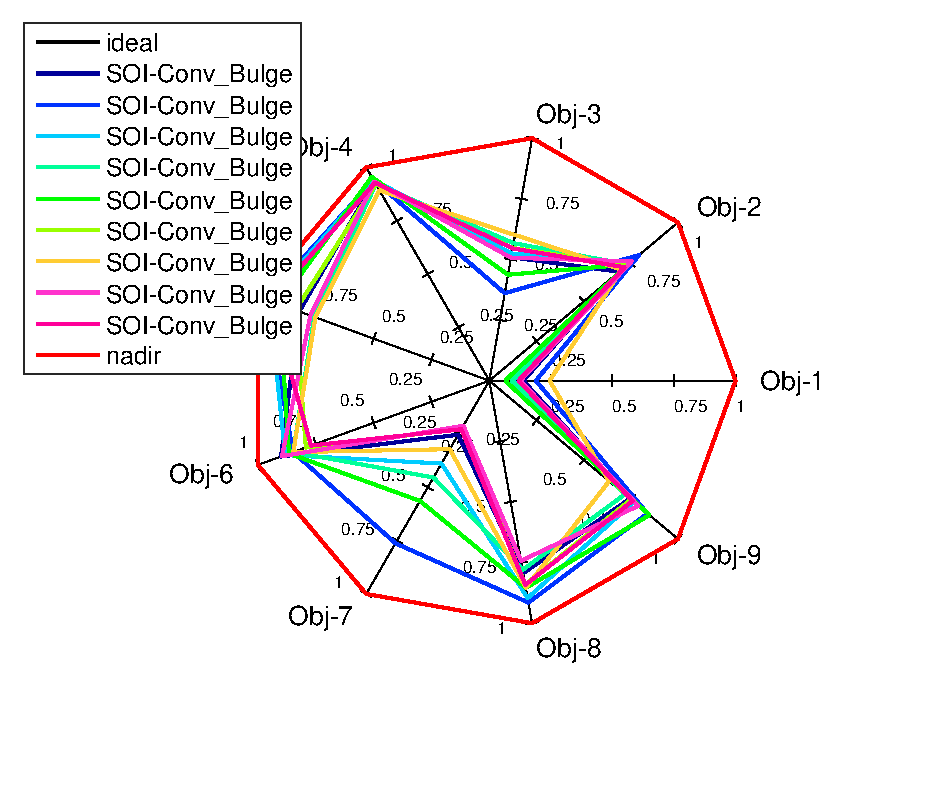
\includegraphics[width=0.37\textwidth]{Figures/Figure25.eps}}
	\subfigure[]{\label{fig:reducerad}\includegraphics[width=0.37\textwidth]{Figures/Figure26.eps}}      
	\caption{Radar: (a) EMU\textsuperscript{r}, (b) EMU, (c) Convex Bulge, (d) SOIs}
	\label{fig:radarplot}
\end{figure*}

\begin{itemize}
	\setlength\itemsep{0em}
	\item It is interesting to note that in the scaled objective space, 46\% of the points have negative distance values~(i.e., they lie in the region towards the nadir point) from the hyperplane, which indicates that it is a mixed~(convex+concave) front in global sense. The maximum distances from hyperplane towards the ideal point and nadir point in the scaled space are 0.0731 units and 0.1573 units respectively. Therefore, the non-convex part is relatively farther from hyperplane than the convex part.   
	\item Top 9 SOIs in the scaled objective space are presented in Fig.~\ref{fig:radarplot}. It is clear that the SOI\textsubscript{f} selected by the proposed approach are all peripheral solutions. 4 solutions within SOI\textsubscript{f} have at least one objective value minimum among all the points and belong to $Peripheral_E$ class and the rest belong to $Peripheral$ class. It is also important to take note that before the reduction stage, the set SOI contained 9 solutions. Therefore the cardinality of the final set SOI\textsubscript{f} is same as SOI. The solutions identified using the proposed approach are unique and adhere to the resolution inherently defined using the number of given reference directions. They also do not have extreme values unlike solutions selected using other approaches.
	\item  A further visualization of different SOIs and corners in the objective space is shown in Fig.~\ref{fig:reducerad}, wherein multidimensional scaling (MDS) \cite{drtoolbox} was used to transform the original objective space into bi-objective space. For reference, we also include the ``corner'' solutions identified using the method proposed in \cite{singh2011corner}. It can be observed that the $Peripheral/Peripheral_E$ SOI obtained using the proposed approach coincide/lie close to them. The corner solutions are listed in \cite{benchmark}.
	
\end{itemize}

\subsubsection{General aviation aircraft problem}

Next, we consider the 10-objective General aviation aircraft problem introduced in \cite{Simpson1996}. For this problem, decomposition based evolutionary algorithm~(DBEA)~\cite{asafuddoula2014decomposition} was run for 100 generations with a population size of 11,440 to obtain a set of 10928 unique non-dominated solutions. The number of reference directions used for EMU\textsuperscript{r} and EMU computations was set to 5005. Fig.~\ref{fig:gaaplot} represents SOIs obtained using various approaches (except HV contribution based measure since it is computationally prohibitive for such high number of data points with 10 objectives). The observations can be summarized as follows:

\begin{figure*}[!htb]
	\centering    
	\subfigure[]{\label{fig:remugaa}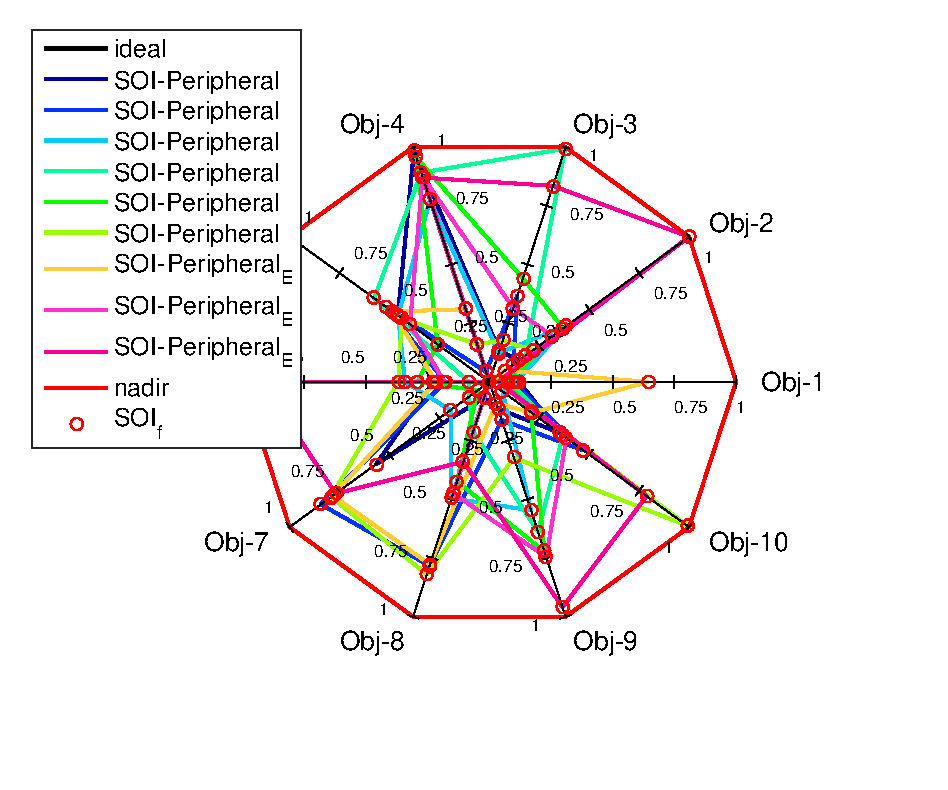
\includegraphics[width=0.37\textwidth]{Figures/Figure27.eps}}
	\subfigure[]{\label{fig:emugaa}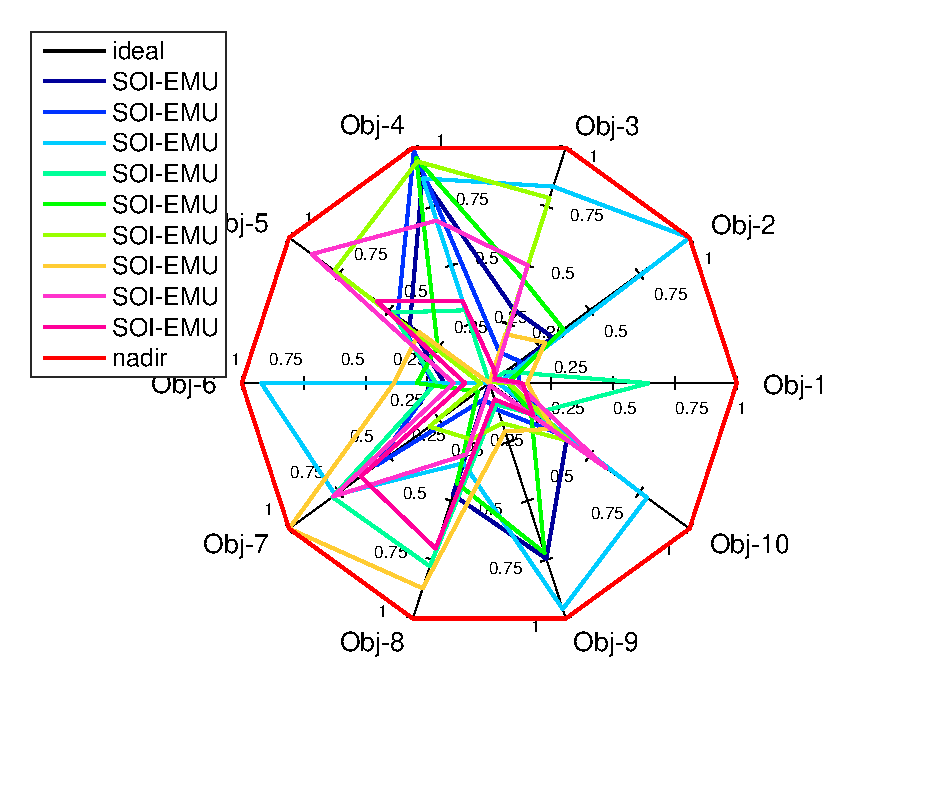
\includegraphics[width=0.37\textwidth]{Figures/Figure28.eps}}
	\subfigure[]{\label{fig:hypgaa}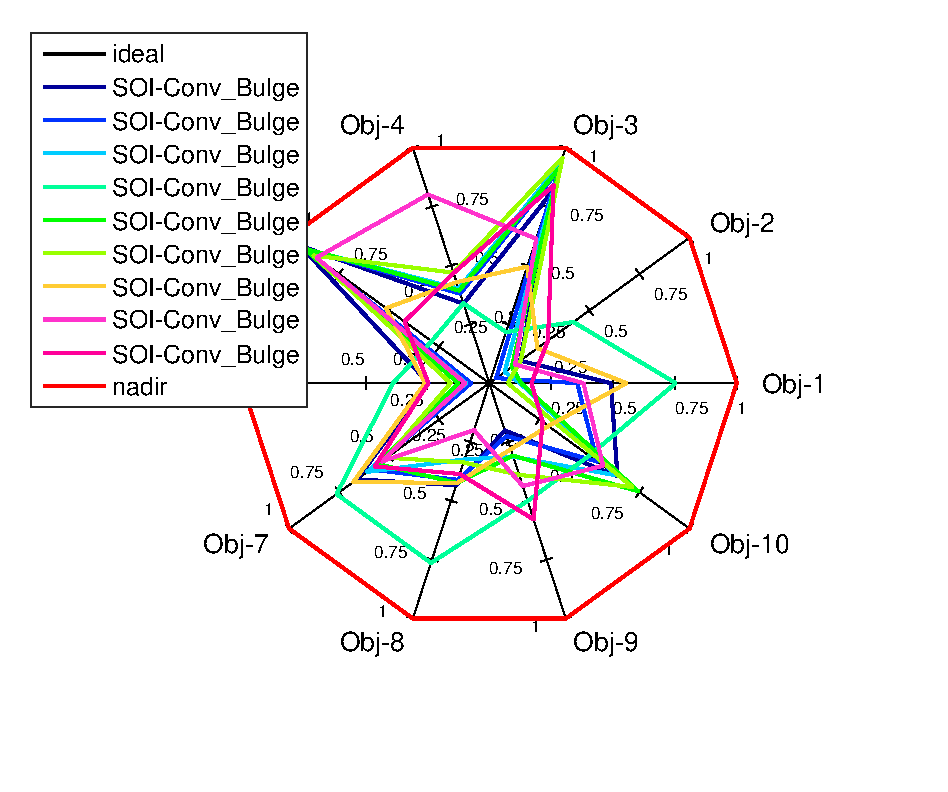
\includegraphics[width=0.37\textwidth]{Figures/Figure29.eps}} 
	\subfigure[]{\label{fig:reducegaa}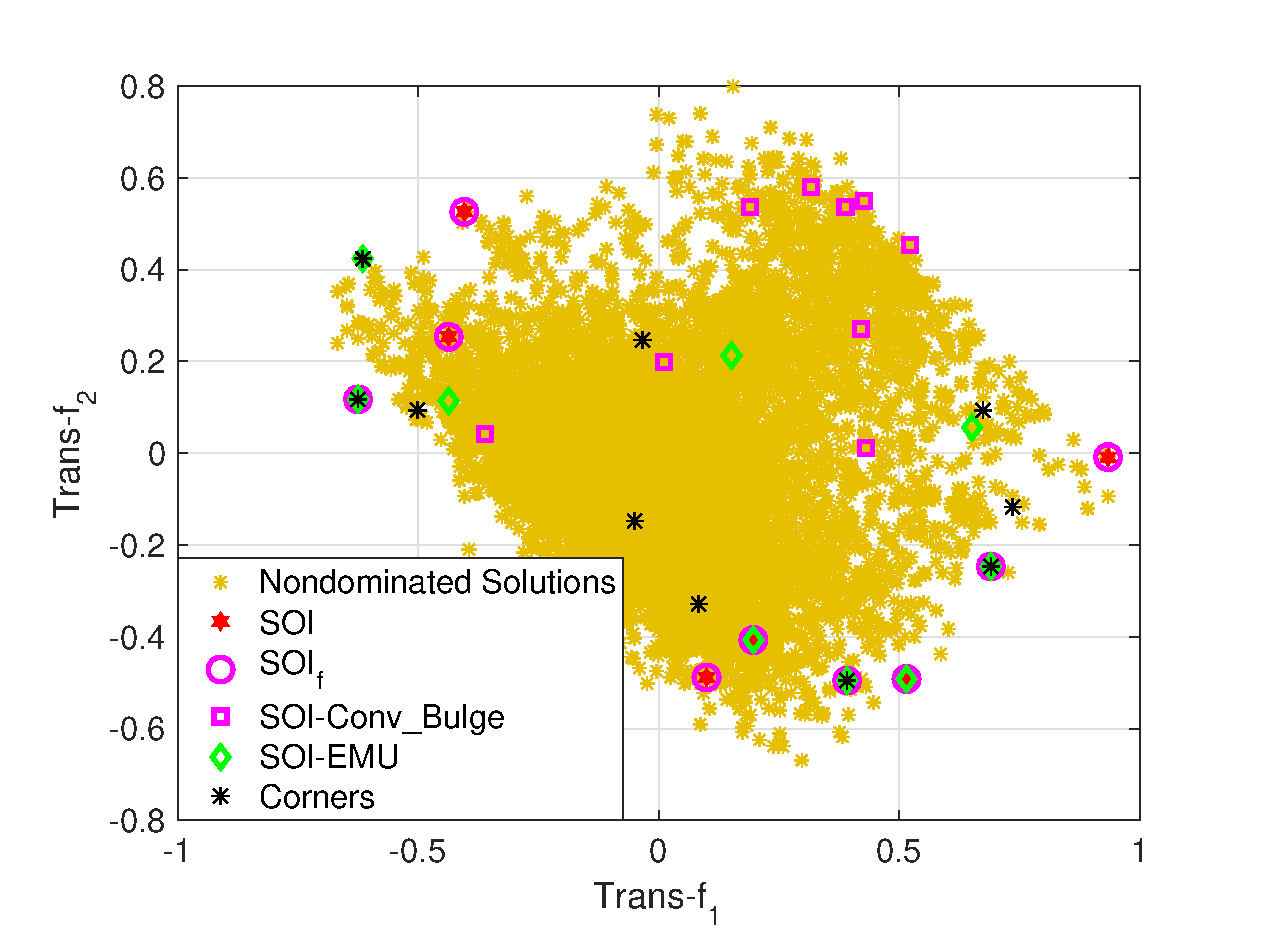
\includegraphics[width=0.37\textwidth]{Figures/Figure30.eps}}      
	\caption{GAA: (a) EMU\textsuperscript{r}, (b) EMU, (c) Convex Bulge, (d) SOIs}
	\label{fig:gaaplot}
\end{figure*}

\begin{itemize}
	\setlength\itemsep{0em}
	\item The distances from hyperplane values have mixed~(positive/negative) signs, which indicates that the non-dominated front is a combination of convex and non-convex regions. In the scaled objective space, the maximum positive distance is 0.1840~(towards ideal point) and 0.2581 towards the nadir. About 59\% of the points have negative distance values i.e., towards the nadir point. 
	\item SOI contains 6 solutions belonging to $Peripheral$ class and 3 solutions belonging to $Peripheral_E$ class before the reduction stage. Therefore, the cardinality of SOI\textsubscript{f} is same as SOI.
	\item Top 9 solutions of interest~(SOI) in terms of EMU and convex bulge are presented in Fig.~\ref{fig:emugaa} and Fig.~\ref{fig:hypgaa} respectively in the scaled objective space.  
	\item The SOIs obtained using different measures and the corners are shown in Fig.~\ref{fig:reducegaa} in transformed bi-objective space using MDS. The corners of the non-dominated set of solutions obtained using Pareto-corner sort \cite{singh2011corner} are also shown for comparison. Once again, it can be seen that they coincide/lie close to the obtained SOIs. The corner solutions are listed in \cite{benchmark}.   
\end{itemize} 

Due to space limitations, additional analysis of the solutions obtained for GAA and radar waveform design is included in the supplementary material~(also available on authors' website~\cite{benchmark}).
\section{Online use of the proposed measure}
In the examples above, we have illustrated the utility of the measure to identify solutions of interest \textit{a posteriori}. Now we illustrate its use to guide an optimization algorithm towards potential regions containing SOIs. To this end we have used the EMU\textsuperscript{r} in conjunction with DBEA~\cite{asafuddoula2014decomposition} for DEB3DK with 4 knee regions. We used the same number of reference directions and population size~(300) as discussed above for this problem and allowed it to evolve over 1200 generations. For this experiment, $K$ is set \emph{equal} to the population size, in order to focus the search towards the SOI. Fig.~\ref{fig:deb3dk4dbea} shows the final population which clearly indicates greater intensity of solutions in the regions of interest. 

\begin{figure}[!htb]
	\centering    
	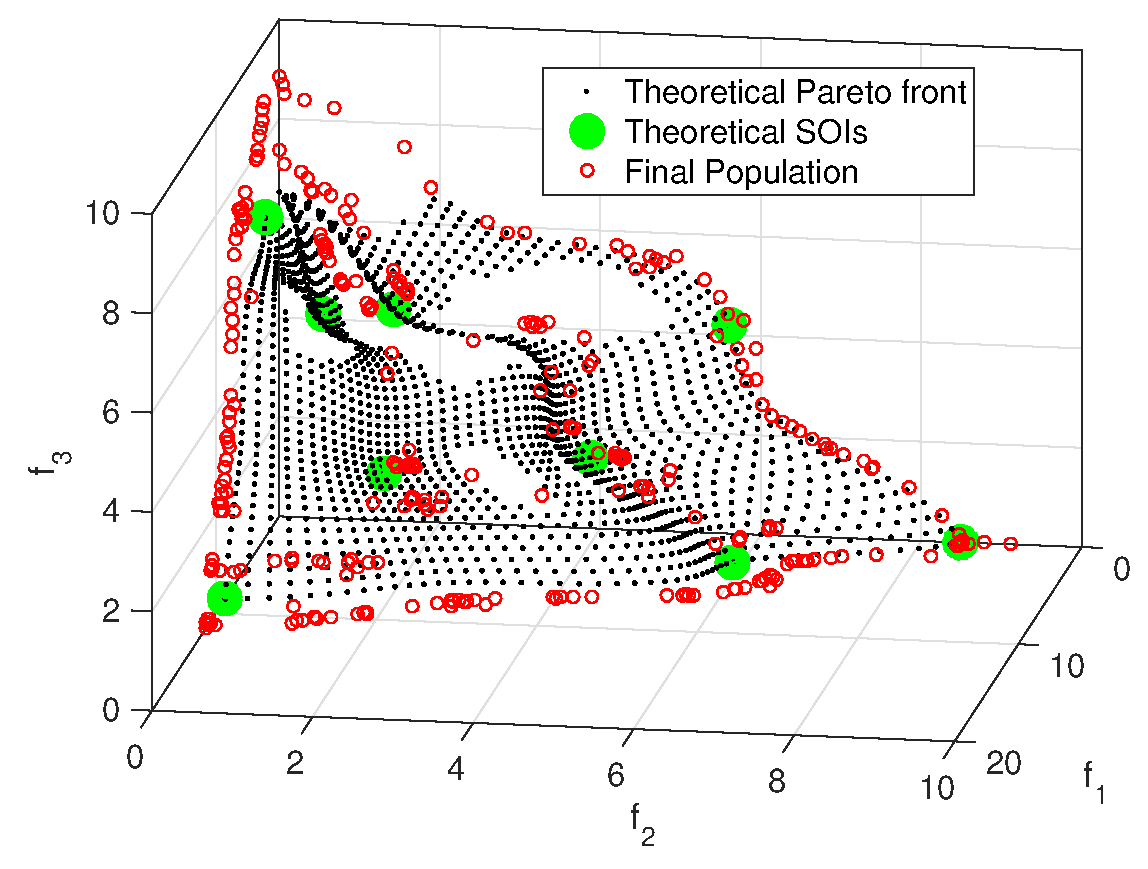
\includegraphics[width=0.28\textwidth]{Figures/Figure31.eps} 
	\caption{Online identification of SOIs}
	\label{fig:deb3dk4dbea}
\end{figure}

\section{Conclusions}
\label{sec:sum}
Multi-/many-objective optimization algorithms typically deliver a set of trade-off solutions as their output. Since the size of these sets is often very large~(containing potentially several thousand solutions), choosing one~(or a few solutions) for final implementation is a significantly challenging problem. In absence of any prior knowledge/preferences, additional measures are required to identify potential solutions of interest~(SOI). This paper reviews the existing measures in this regard and illustrates that the choice of solutions could vary significantly based on the underlying measure. It also highlights some of their shortcomings, and follows up with a proposal to select solutions of interest based on recursive expected marginal utility computation. The local and global nature of the trade-off surface is also analyzed using convex bulge, EMU and HV contribution based measures. The proposed method inherits the advantages of expected marginal utility for selection, and at the same time delivers diverse SOIs. A further characterization is done on the type of SOI~(internal/peripheral) to aid decision-making. It is also important to take note that the relative importance of the selected solutions is inherently available through this process. An illustration of its \emph{online} utility to intensify the search around SOIs is also presented. We hope this study would encourage further research in this direction which could bridge the gap between ``generation of the trade-off set of solutions'' and ``supporting a human decision maker to select solutions for closer examination''. The development of such methods will facilitate increased adoption of multi-/many-objective optimization algorithms for solving real-world problems. 

